\chapter{Analisis}
\label{chap:analisis}

Pada bab ini akan dijelaskan analisis mengenai hasil wawancara, hasil kuesioner, nama baptis berdasarkan metode SAW, nama baptis berdasarkan metode SAW menggunakan database, dan perangkat lunak berupa \textit{use case}.

\section{Analisis Hasil Wawancara}
\label{sec:analisiswawancara}

Dalam menganalisis kebutuhan pemilihan nama baptis Katolik, peneliti melakukan wawancara dengan Pastor Paroki St. Laurentius, A. Boogaarts, OSC (Lampiran \ref{fig:bukti}). Wawancara dengan Pastor Paroki bertujuan untuk mengetahui secara mendetail atau terperinci mengenai pembaptisan dalam agama Katolik. Setelah melakukan wawancara, penulis mendapatkan penjelasan secara umum mengenai Baptis, nama Baptis, serta cara pemilihan nama Baptis.
\begin{enumerate}
	\item Makna baptis untuk agama Katolik adalah suatu lambang lahiriah di mana diungkapkan, bahwa menjadi anggota gereja Katolik yang secara resmi adalah diangkat menjadi anak Allah.
	\item Tidak harus ada nama baptis. Tetapi nama baptis merupakan suatu tradisi sebagai ungkapan bahwa di dalam baptisan itu dikuduskan dengan harapan tidak sembarangan memilih nama baptis, tetapi lebih ingin meniru teladan orang kudus yang dia pilih sebagai nama baptis, sehingga menjadi kudus dengan nama baptis yang dia pilih.
		%\item Cara pembaptisan dalam agama Katolik selain disiram dengan air adalah ditenggelamkan/ dibenamkan/ dicelupkan menggunakan air yang mengalir yang telah diberkati (air percikan tidak cukup).
		%\item Ada beberapa kelemahan ketika baptis waktu bayi, yaitu kurangnya mendapatkan pendalaman iman. Tetapi ada keuntungannya juga, yaitu telah mengikut Yesus Kristus dari sewaktu Bayi. Sedangkan jika baptis dewasa, yaitu benar-benar belajar dengan cara mencari komunitas/ dapat membantu dia memilih Yesus Kristus sebagai Juru Selamat serta Kitab Suci dan sebagainya.
		\item Pemilihan nama baptis tidak ada kriteria (bebas memilih), tetapi sebaiknya kita memilih orang yang sekiranya dekat dengan bakat kita/ nama karena mirip/ karena artinya. Tanggal, tanggal pembaptisan serta pesta nama baptis juga bisa dijadikan acuan dalam memilih nama baptis.
\end{enumerate}

		Penelitian ini berfokus pada pembahasan pemilihan nama baptis, untuk itu bagian yang akan dianalisa lebih mendalam adalah pada bagian kriteria pemilihan nama Baptis. Berdasarkan hasil wawancara di atas, dapat dianalisa bahwa nama baptis tidak diharuskan, tetapi nama baptis sudah merupakan sebuah tradisi dalam agama Katolik. Kriteria pemilihan nama baptis yang bisa dijadikan sebuah acuan atau pedoman dalam memilih nama Baptis berdasarkan hasil wawancara adalah sebagai berikut:
	
	\begin{itemize}
		\item Bakat calon Baptis (profesi)
		\item Nama calon Baptis
		\item Tanggal lahir calon Baptis
		\item Tanggal pembaptisan calon Baptis
		\item Tanggal Pesta santo-santa (tanggal peringatan)
		\item Arti santo-santa
	\end{itemize}


\section{Analisis Hasil Kuesioner}
\label{sec:analisiskuesioner}

Dalam menganalisis kebutuhan pemilihan nama baptis Katolik, peneliti menyebarkan kuesioner yang telah dibuat dengan menggunakan Google Form. Pada Google Form, terdapat lima pertanyaan. Berikut adalah pertanyaan dari formulir kuesioner pemilihan nama baptis Katolik (Lampiran \ref{fig:form}).


\begin{enumerate}
	\item Apakah anda seorang Katolik?
	
	Pertanyaan ini dibuat dengan tujuan agar penulis dapat mengetahui persentase \textit{user} yang mengisi beragama Katolik atau calon Katolik. Yang dimaksud calon Katolik adalah orang yang ingin masuk ke dalam agama Katolik atau mengikuti Kristus sebagai Juru Selamat-Nya. Penulis memberikan sebuah pilihan untuk jawaban pertanyaan ini, yaitu ya dan tidak. Jika \textit{user} mengisi dan jawabannya adalah ya, maka \textit{user} dapat membantu dalam hal analisis kebutuhan pemilihan nama baptis. %Jika \textit{user} mengisi dan jawabannya adalah Tidak, maka \textit{user} dapat menambah pengetahuan \textit{user} mengenai pemilihan nama baptis. 
	\item Jika jawaban anda Ya, apakah anda sudah dibaptis?
	
	Pertanyaan ini dibuat dengan tujuan agar penulis dapat mengetahui persentase \textit{user} yang sudah dibaptis. Penulis memberikan sebuah pilihan untuk jawaban pertanyaan ini, yaitu sudah dan belum. Jika \textit{user} mengisi dan jawabannya adalah sudah, maka \textit{user} dapat membantu dalam hal analisis kebutuhan pemilihan nama baptis. %Jika penulis sudah mengetahui presentasi yang dibaptis, maka dapat membantu dalam hal analisis kebutuhan pemilihan nama baptis.
	\item Jika sudah, kapan anda telah dibaptis?
	
	Pertanyaan ini dibuat dengan tujuan agar penulis dapat mengetahui persentase \textit{user} yang sudah dibaptis ketika bayi dan juga ketika dewasa. Penulis memberikan sebuah pilihan untuk jawaban pertanyaan ini, yaitu ketika masih bayi dan ketika sudah dewasa.
	%\item Apa yang membuat anda dibaptis?
	
	%Pertanyaan ini dibuat dengan tujuan agar penulis dapat mengetahui alasan yang membuat \textit{user} ingin dibaptis. Jawaban pertanyaan ini berupa teks kosong, sehingga \textit{user} dapat mengisi beberapa alasan secara bebas.
	\item Anda memilih nama baptis tersebut berdasarkan apa saja?
	
	Pertanyaan ini dibuat dengan tujuan agar penulis dapat mengetahui faktor yang patut untuk dijadikan sebagai sebuah kriteria pemilihan nama baptis Katolik. Penulis memberikan beberapa pilihan untuk jawaban pertanyaan ini, yaitu tanggal lahir, tanggal pembaptisan Anda, deskripsi santo-santa (cerita kehidupan santo-santa), tanggal pesta santo-santa (peringatan), profesi santo-santa, arti nama dari santo-santa, lambang dari santo-santa, dan jika \textit{user} ingin menjawab selain pilihan tersebut. Jawaban dengan pilihan yang lain juga dapat dijadikan sebuah kriteria, jika jawabannya masuk akal.
\end{enumerate}

Penelitian ini berfokus pada pembahasan pemilihan nama baptis, untuk itu bagian yang akan dianalisa lebih mendalam adalah pada bagian kriteria pemilihan nama Baptis. Sampel yang diambil adalah seratus orang yang terdiri dari 96 orang beragama Katolik dan 4 orang calon Katolik (Lampiran \ref{fig:kues1}, Lampiran \ref{fig:kues2}, Lampiran \ref{fig:kues3}, Lampiran \ref{fig:kues4}, Lampiran \ref{fig:kues5}, Lampiran \ref{fig:kues6}). Setiap responden ada yang memilih kriteria nama baptis sampai 4 atau 5 kategori. Kriteria pemilihan nama baptis yang bisa dijadikan sebuah acuan atau pedoman dalam memilih nama Baptis berdasarkan hasil kuesioner adalah sebagai berikut (Gambar \ref{fig:Capture}):

\begin{itemize}
			\item Tanggal Lahir sebanyak 11 \textit{user}.
			\item Tangal Pembaptisan sebanyak 6 \textit{user}.
			\item Deskripsi atau cerita kehidupan Santo-Santa sebanyak 32 \textit{user}.
			\item Pesta Santo-Santa sebanyak 1 \textit{user}.
			\item Profesi Santo-Santa sebanyak 6 \textit{user}.
			\item Arti Nama Santo-Santa sebanyak 45 \textit{user}.
			\item Lambang dari Santo-Santa sebanyak 5 \textit{user}.
			\item Lain-lain sebanyak 26 \textit{user}.
		\end{itemize}
		
	\begin{figure}[htbp]
		\centering
			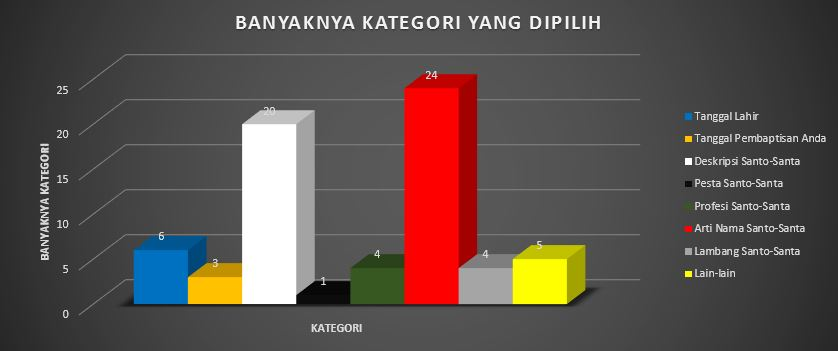
\includegraphics[scale=0.7]{Gambar/Capture.JPG}
			\caption{Kategori Pemilihan Nama Baptis}
		\label{fig:Capture}
	\end{figure}

	Dengan demikian, berdasarkan hasil kuesioner di atas (Gambar \ref{fig:Capture}), dapat di analisa bahwa kriteria yang paling banyak dijadikan acuan atau pedoman (diurutkan berdasarkan responden terbanyak) adalah sebagai berikut:
	
	\begin{itemize}
		\item Kriteria pertama \\
		Arti Nama Santo-Santa dengan jumlah responden 45 \textit{user}.
		\item Kriteria kedua \\
		Deskripsi atau cerita kehidupan Santo-Santa dengan jumlah responden 32 \textit{user}.
		\item Kriteria ketiga \\
		Tanggal lahir calon Baptis dengan jumlah responden 11 \textit{user}.
		\item Kriteria keempat \\
		Tanggal pembaptisan dan profesi Santo-Santa dengan jumlah responden 6 \textit{user}.
		\item Kriteria kelima\\
		Lambang Santo-Santa dengan jumlah responden 5 \textit{user}.
		\item Kriteria keenam\\
		Tanggal pesta Santo-Santa dengan jumlah responden 1 \textit{user}.
	\end{itemize}
	

\section{Analisis Nama Baptis }
\label{sec:analisisnb}

\subsection{Analisis SAW}
\label{sec:analisissaw}
	
	Berdasarkan hasil analisis pada subbab \ref{sec:analisiswawancara} dan subbab \ref{sec:analisiskuesioner}, didapatkan beberapa kriteria dalam memilih nama baptis pada agama Katolik. Terdapat 7 kriteria $C_{i}$ yang digunakan untuk menentukan nama baptis yang tepat untuk calon baptis. Kriteria diperlukan oleh calon baptis, agar calon baptis dapat menentukan nama baptis yang dijadikan sebagai nama alternatif tersebut. Berikut 7 kriteria yang telah ditentukan berdasarkan hasil analisa wawancara dan kuesioner:
\begin{enumerate}
	\item $C_{1}$ = Arti nama santo-santa
	\item $C_{2}$ = Deskripsi atau cerita kehidupan santo-santa
	\item $C_{3}$ = Tanggal lahir calon baptis
	\item $C_{4}$ = Tanggal pembaptisan
	\item $C_{5}$ = Profesi santo-santa
	\item $C_{6}$ = Lambang santo-santa
	\item $C_{7}$ = Tanggal pesta santo-santa
\end{enumerate}
	
		Pada beberapa kriteria yang sudah ditentukan akan diberikan bobot pada masing-masing kriteria. Bobot ($W_{j}$) untuk setiap kriteria adalah sebagai berikut:
		
\begin{enumerate}
	\item $C_{1}$ = 40\% = 0.4
	\item $C_{2}$ = 20\% = 0.2
	\item $C_{3}$ = 10\% = 0.1
	\item $C_{4}$ = 15\% = 0.15
	\item $C_{5}$ = 5\% = 0.05
	\item $C_{6}$ = 5\% = 0.05
	\item $C_{7}$ = 5\% = 0.05
\end{enumerate}

Selain terdapat kriteria, metode SAW juga membutuhkan sebuah alternatif $A_{i}$. Alternatif pada pemilihan nama baptis Katolik adalah nama santo-santa. Ada 10 nama santo-santa yang menjadi nama alternatif untuk dijadikan nama baptis yang tepat oleh calon baptis. Pada pemilihan nama baptis, alternatif tersebut termasuk dalam atribut keuntungan (\textit{benefit}), karena hasil \textit{output} yang akan dikeluarkan adalah menguntungkan calon baptis tersebut.

\begin{enumerate}
	\item $A_{1}$ = Abraham
	\item $A_{2}$ = Adam
	\item $A_{3}$ = Adolf
	\item $A_{4}$ = Agata
	\item $A_{5}$ = Agnes
	\item $A_{6}$ = Agustinus
	\item $A_{7}$ = Brigitta
	\item $A_{8}$ = Daud
	\item $A_{9}$ = Natalia
	\item $A_{10}$ = Yoakim
\end{enumerate}

Pada metode SAW membutuhkan proses normalisasi. Proses normalisasi adalah proses pengelompokkan data berdasarkan atribut. Pada pemilihan nama baptis, data dikelompokkan berdasarkan atribut keuntungan (\textit{benefit}). Pada setiap alternatif yang telah dikelompokkan tersebut, diberikan sebuah angka atau nilai. Angka atau nilai tersebut didapatkan dari hasil \textit{input user} pada kriteria yang ditentukan. Rentang nilai pada masing-masing alteratif pada setiap kata yang dicari adalah 0 sampai 100. Berikut adalah tabel nilai alternatif pada setiap kriteria:

\begin{table}[H]
	\centering
	\caption{Tabel Nilai Alternatif Analisis SAW}
		\begin{tabular}{|l|r|r|r|r|r|r|r|} \hline
		 Alternatif    & $C_{1}$ & $C_{2}$ & $C_{3}$ & $C_{4}$ & $C_{5}$ & $C_{6}$ & $C_{7}$ \\
    \hline
    Abraham     & 5&5&5&5&5&5&5     \\ \hline
    Adam	      & 5&5&90&90&5&5&90    \\ \hline
    Adolf       & 5&5&5&5&45&5&5      \\ \hline
    Agata       & 15&30&15&15&15&90&15  \\ \hline
		Agnes    		& 90&30&20&20&20&20&20     \\ \hline
    Agustinus	  & 20&30&20&20&45&20&20    \\ \hline
    Brigitta    & 5&5&5&5&5&5&5      \\ \hline
    Daud       	& 10&10&45&45&10&10&45  \\ \hline
		Natalia     & 25&25&25&25&25&25&25      \\ \hline
    Yoakim      & 5&5&5&5&5&5&5  \\ \hline
				\end{tabular}
	\label{table:nilaialternatifsaw}
\end{table}


Dari data yang sudah didapatkan sebelumnya, maka permasalahan pengambilan keputusan calon baptis dapat diselesaikan. Untuk menyelesaikan permasalahan tersebut dibutuhkan penormalisasian. Berikut adalah rumus normalisasi:
	\[ r_{ij}  =
  \begin{cases}
    \frac{x_{ij}}{\stackrel{Max}{i} x_{ij}}      & \quad \text{jika } j \text{ adalah atribut keuntungan (\textit{benefit})}\\
	\end{cases}	  
\]

Perhitungan dilakukan untuk masing-masing kriteria pada setiap alternatif. Perhitungan dilakukan dengan cara mengambil $x_{ij}$ pada bagian kolom kriteria $C_{i}$ dan nilai maximum (${\stackrel{Max}{i} x_{ij}}$) dari masing-masing kolom pada setiap kriteria. Berikut adalah cara untuk menormalisasikan pada masing-masing kriteria.

\begin{enumerate}
%kolom 1
	\item Pada $C_{1}$ penyelesaiannya sebagai berikut:
\begin{displaymath}
r_{11} = \frac{5}{max {5;5;5;15;90;20;5;10;25;5}} = \frac{5}{90} = 0.05\\
\end {displaymath}
\begin{displaymath}
r_{21} = \frac{5}{max {5;5;5;15;90;20;5;10;25;5}} = \frac{5}{90} = 0.05\\
\end{displaymath}
\begin{displaymath}
r_{31} = \frac{5}{max {5;5;5;15;90;20;5;10;25;5}} = \frac{5}{90} = 0.05\\
\end {displaymath}
\begin{displaymath}
r_{41} = \frac{15}{max {5;5;5;15;90;20;5;10;25;5}} = \frac{15}{90} = 0.16\\
\end {displaymath}
\begin{displaymath}
r_{51} = \frac{90}{max {5;5;5;15;90;20;5;10;25;5}} = \frac{90}{90} = 1\\
\end {displaymath}
\begin{displaymath}
r_{61} = \frac{20}{max {5;5;5;15;90;20;5;10;25;5}} = \frac{20}{90} = 0.22\\
\end {displaymath}
\begin{displaymath}
r_{71} = \frac{5}{max {5;5;5;15;90;20;5;10;25;5}} = \frac{5}{90} = 0.05\\
\end {displaymath}
\begin{displaymath}
r_{81} = \frac{10}{max {5;5;5;15;90;20;5;10;25;5}} = \frac{10}{90} = 0.11\\
\end {displaymath}
\begin{displaymath}
r_{91} = \frac{25}{max {5;5;5;15;90;20;5;10;25;5}} = \frac{25}{90} = 0.27\\
\end {displaymath}
\begin{displaymath}
r_{101} = \frac{5}{max {5;5;5;15;90;20;5;10;25;5}} = \frac{5}{90} = 0.05\\
\end {displaymath}

%kolom 2
\item Pada $C_{2}$ penyelesaiannya sebagai berikut:
\begin{displaymath}
r_{12} = \frac{5}{max {5;5;5;30;30;30;5;10;25;5}} = \frac{5}{30} = 0.16\\
\end {displaymath}
\begin{displaymath}
r_{22} = \frac{5}{max {5;5;5;30;30;30;5;10;25;5}} = \frac{5}{30} = 0.16\\
\end{displaymath}
\begin{displaymath}
r_{32} = \frac{5}{max {5;5;5;30;30;30;5;10;25;5}} = \frac{5}{30} = 0.16\\
\end {displaymath}
\begin{displaymath}
r_{42} = \frac{30}{max {5;5;5;30;30;30;5;10;25;5}} = \frac{30}{30} = 1\\
\end {displaymath}
\begin{displaymath}
r_{52} = \frac{30}{max {5;5;5;30;30;30;5;10;25;5}} = \frac{30}{30} = 1\\
\end {displaymath}
\begin{displaymath}
r_{62} = \frac{30}{max {5;5;5;30;30;30;5;10;25;5}} = \frac{30}{30} = 1\\
\end {displaymath}
\begin{displaymath}
r_{72} = \frac{5}{max {5;5;5;30;30;30;5;10;25;5}} = \frac{5}{30} = 0.16\\
\end {displaymath}
\begin{displaymath}
r_{82} = \frac{10}{max {5;5;5;30;30;30;5;10;25;5}} = \frac{10}{30} = 0.33\\
\end {displaymath}
\begin{displaymath}
r_{92} = \frac{25}{max {5;5;5;30;30;30;5;10;25;5}} = \frac{25}{30} = 0.83\\
\end {displaymath}
\begin{displaymath}
r_{102} = \frac{5}{max {5;5;5;30;30;30;5;10;25;5}} = \frac{5}{30} = 0.16\\
\end {displaymath}

%kolom 3
\item Pada $C_{3}$ penyelesaiannya sebagai berikut:
\begin{displaymath}
r_{13} = \frac{5}{max {5;90;5;15;20;20;5;45;25;5}} = \frac{5}{90} = 0.05\\
\end {displaymath}
\begin{displaymath}
r_{23} = \frac{90}{max {5;90;5;15;20;20;5;45;25;5}} = \frac{90}{90} = 1\\
\end{displaymath}
\begin{displaymath}
r_{33} = \frac{5}{max {5;90;5;15;20;20;5;45;25;5}} = \frac{5}{90} = 0.05\\
\end {displaymath}
\begin{displaymath}
r_{43} = \frac{15}{max {5;90;5;15;20;20;5;45;25;5}} = \frac{15}{90} = 0.16\\
\end {displaymath}
\begin{displaymath}
r_{53} = \frac{20}{max {5;90;5;15;20;20;5;45;25;5}} = \frac{20}{90} = 0.22\\
\end {displaymath}
\begin{displaymath}
r_{63} = \frac{20}{max {5;90;5;15;20;20;5;45;25;5}} = \frac{20}{90} = 0.22\\
\end {displaymath}
\begin{displaymath}
r_{73} = \frac{5}{max {5;90;5;15;20;20;5;45;25;5}} = \frac{5}{90} = 0.05\\
\end {displaymath}
\begin{displaymath}
r_{83} = \frac{45}{max {5;90;5;15;20;20;5;45;25;5}} = \frac{45}{90} = 0.5\\
\end {displaymath}
\begin{displaymath}
r_{93} = \frac{25}{max {5;90;5;15;20;20;5;45;25;5}} = \frac{25}{90} = 0.27\\
\end {displaymath}
\begin{displaymath}
r_{103} = \frac{5}{max {5;90;5;15;20;20;5;45;25;5}} = \frac{5}{90} = 0.05\\
\end {displaymath}
%kolom 4
\item Pada $C_{4}$ penyelesaiannya sebagai berikut:
\begin{displaymath}
r_{14} = \frac{5}{max {5;90;5;15;20;20;5;45;25;5}} = \frac{5}{90} = 0.05\\
\end {displaymath}
\begin{displaymath}
r_{24} = \frac{90}{max {5;90;5;15;20;20;5;45;25;5}} = \frac{90}{90} = 1\\
\end{displaymath}
\begin{displaymath}
r_{34} = \frac{5}{max {5;90;5;15;20;20;5;45;25;5}} = \frac{5}{90} = 0.05\\
\end {displaymath}
\begin{displaymath}
r_{44} = \frac{15}{max {5;90;5;15;20;20;5;45;25;5}} = \frac{15}{90} = 0.16\\
\end {displaymath}
\begin{displaymath}
r_{54} = \frac{20}{max {5;90;5;15;20;20;5;45;25;5}} = \frac{20}{90} = 0.22\\
\end {displaymath}
\begin{displaymath}
r_{64} = \frac{20}{max {5;90;5;15;20;20;5;45;25;5}} = \frac{20}{90} = 0.22\\
\end {displaymath}
\begin{displaymath}
r_{74} = \frac{5}{max {5;90;5;15;20;20;5;45;25;5}} = \frac{5}{90} = 0.05\\
\end {displaymath}
\begin{displaymath}
r_{84} = \frac{45}{max {5;90;5;15;20;20;5;45;25;5}} = \frac{45}{90} = 0.5\\
\end {displaymath}
\begin{displaymath}
r_{94} = \frac{25}{max {5;90;5;15;20;20;5;45;25;5}} = \frac{25}{90} = 0.27\\
\end {displaymath}
\begin{displaymath}
r_{104} = \frac{5}{max {5;90;5;15;20;20;5;45;25;5}} = \frac{5}{90} = 0.05\\
\end {displaymath}

%kolom 5
\item Pada $C_{5}$ penyelesaiannya sebagai berikut:
\begin{displaymath}
r_{15} = \frac{5}{max {5;5;45;15;20;45;5;10;25;5}} = \frac{5}{45} = 0.11\\
\end {displaymath}
\begin{displaymath}
r_{25} = \frac{5}{max {5;5;45;15;20;45;5;10;25;5}} = \frac{5}{45} = 0.11\\
\end{displaymath}
\begin{displaymath}
r_{35} = \frac{45}{max {5;5;45;15;20;45;5;10;25;5}} = \frac{45}{45} = 1\\
\end {displaymath}
\begin{displaymath}
r_{45} = \frac{15}{max {5;5;45;15;20;45;5;10;25;5}} = \frac{15}{45} = 0.33\\
\end {displaymath}
\begin{displaymath}
r_{55} = \frac{20}{max {5;5;45;15;20;45;5;10;25;5}} = \frac{20}{45} = 0.44\\
\end {displaymath}
\begin{displaymath}
r_{65} = \frac{45}{max {5;5;45;15;20;45;5;10;25;5}} = \frac{45}{45} = 1\\
\end {displaymath}
\begin{displaymath}
r_{75} = \frac{5}{max {5;5;45;15;20;45;5;10;25;5}} = \frac{5}{45} = 0.11\\
\end {displaymath}
\begin{displaymath}
r_{85} = \frac{10}{max {5;5;45;15;20;45;5;10;25;5}} = \frac{10}{45} = 0.22\\
\end {displaymath}
\begin{displaymath}
r_{95} = \frac{25}{max {5;5;45;15;20;45;5;10;25;5}} = \frac{25}{45} = 0.55\\
\end {displaymath}
\begin{displaymath}
r_{105} = \frac{5}{max {5;5;45;15;20;45;5;10;25;5}} = \frac{5}{45} = 0.11\\
\end {displaymath}
%kolom 6
\item Pada $C_{6}$ penyelesaiannya sebagai berikut:
\begin{displaymath}
r_{16} = \frac{5}{max {5;5;5;90;20;20;5;10;25;5}} = \frac{5}{90} = 0.05\\
\end {displaymath}
\begin{displaymath}
r_{26} = \frac{5}{max {5;5;5;90;20;20;5;10;25;5}} = \frac{5}{90} = 0.05\\
\end{displaymath}
\begin{displaymath}
r_{36} = \frac{5}{max {5;5;5;90;20;20;5;10;25;5}} = \frac{5}{90} = 0.05\\
\end {displaymath}
\begin{displaymath}
r_{46} = \frac{90}{max {5;5;5;90;20;20;5;10;25;5}} = \frac{90}{90} = 1\\
\end {displaymath}
\begin{displaymath}
r_{56} = \frac{20}{max {5;5;5;90;20;20;5;10;25;5}} = \frac{20}{90} = 0.22\\
\end {displaymath}
\begin{displaymath}
r_{66} = \frac{20}{max {5;5;5;90;20;20;5;10;25;5}} = \frac{20}{90} = 0.22\\
\end {displaymath}
\begin{displaymath}
r_{76} = \frac{5}{max {5;5;5;90;20;20;5;10;25;5}} = \frac{5}{90} = 0.05\\
\end {displaymath}
\begin{displaymath}
r_{86} = \frac{10}{max {5;5;5;90;20;20;5;10;25;5}} = \frac{10}{90} = 0.11\\
\end {displaymath}
\begin{displaymath}
r_{96} = \frac{25}{max {5;5;5;90;20;20;5;10;25;5}} = \frac{25}{90} = 0.27\\
\end {displaymath}
\begin{displaymath}
r_{106} = \frac{5}{max {5;5;5;90;20;20;5;10;25;5}} = \frac{5}{90} = 0.05\\
\end {displaymath}
%kolom 7
\item Pada $C_{7}$ penyelesaiannya sebagai berikut:
\begin{displaymath}
r_{17} = \frac{5}{max {5;90;5;15;20;20;5;45;25;5}} = \frac{5}{90} = 0.05\\
\end {displaymath}
\begin{displaymath}
r_{27} = \frac{90}{max {5;90;5;15;20;20;5;45;25;5}} = \frac{90}{90} = 1\\
\end{displaymath}
\begin{displaymath}
r_{37} = \frac{5}{max {5;90;5;15;20;20;5;45;25;5}} = \frac{5}{90} = 0.05\\
\end {displaymath}
\begin{displaymath}
r_{47} = \frac{15}{max {5;90;5;15;20;20;5;45;25;5}} = \frac{15}{90} = 0.16\\
\end {displaymath}
\begin{displaymath}
r_{57} = \frac{20}{max {5;90;5;15;20;20;5;45;25;5}} = \frac{20}{90} = 0.22\\
\end {displaymath}
\begin{displaymath}
r_{67} = \frac{20}{max {5;90;5;15;20;20;5;45;25;5}} = \frac{20}{90} = 0.22\\
\end {displaymath}
\begin{displaymath}
r_{77} = \frac{5}{max {5;90;5;15;20;20;5;45;25;5}} = \frac{5}{90} = 0.05\\
\end {displaymath}
\begin{displaymath}
r_{87} = \frac{45}{max {5;90;5;15;20;20;5;45;25;5}} = \frac{45}{90} = 0.5\\
\end {displaymath}
\begin{displaymath}
r_{97} = \frac{25}{max {5;90;5;15;20;20;5;45;25;5}} = \frac{25}{90} = 0.27\\
\end {displaymath}
\begin{displaymath}
r_{107} = \frac{5}{max {5;90;5;15;20;20;5;45;25;5}} = \frac{5}{90} = 0.05\\
\end {displaymath}
\end{enumerate}

Berikut adalah hasil dari nilai rating kinerja yang sudah ternormalisasi:
\begin{displaymath} R = 
\left (
\begin{array}{rrrrrrr}
0.05 & 0.16 & 0.05 & 0.05 & 0.11 & 0.05 & 0.05\\		
0.05 & 0.16 & 1 & 1 & 0.11 & 0.05 & 1\\
0.05 & 0.16 & 0.05 & 0.05 & 1 & 0.05 &0.05\\
0.16 & 1 & 0.16 & 0.16 & 0.33 & 1 & 0.16\\
1 & 1 & 0.22 & 0.22 & 0.44 & 0.22 & 0.22\\
0.22 & 1 & 0.22 & 0.22 & 1 & 0.22 & 0.22\\
0.05 & 0.16 & 0.05 & 0.05 & 0.11 &0.05 & 0.05\\
0.11 & 0.33 & 0.5 & 0.5 & 0.22 & 0.11 & 0.5\\
0.27 & 0.83 & 0.27 & 0.27 & 0.55 & 0.27 & 0.27\\
0.05 & 0.16 & 0.05 & 0.05 & 0.11 & 0.05 & 0.05\\
			\end{array}\right )	
	\end{displaymath}

Proses normalisasi telah selesai dihitung. Dari hasil proses normalisasi didapatkan hasil berupa beberapa data pada masing-masing alternatif terhadap nilai rating kinerja ($r_{ij}$). Pada setiap kriteria terdapat bobot, yaitu W = [$W_{1}$, $W_{2}$, $W_{3}$, $W_{4}$, $W_{5}$, $W_{6}$, $W_{7}$], yang merepresentasikan W = [0.4, 0.2, 0.1, 0.15, 0.05, 0.05, 0.05]. Untuk mendapatkan nilai akhir ($V_{i}$), maka dibutuhkan rumus preferensi. Dengan rumus preferensi calon baptis dapat menentukan alternatif nama. Berikut adalah rumus preferensi:

\[
 V_{i} =\displaystyle\sum_{j=1}^{n} w_{j} r_{ij}
\]


Perhitungan dilakukan untuk masing-masing alternatif. Berikut adalah cara untuk mendapatkan nilai akhir pada masing-masing alternatif.

\begin{enumerate}
	\item $V_{1}$ = (0.4)(0.05)+(0.2)(0.16)+(0.1)(0.05)+(0.15)(0.05)+(0.05)(0.11)+(0.05)(0.05)+(0.05)(0.05) = 0.02 + 0.032 + 0.005 + 0.0075 + 0.0055 + 0.0025 + 0.0025 = 0.075
	
	\item $V_{2}$ = (0.4)(0.05)+(0.2)(0.16)+(0.1)(1)+(0.15)(1)+(0.05)(0.11)+(0.05)(0.05)+(0.05)(1) = 0.02 + 0.032 + 0.1 + 0.15 + 0.0055 + 0.0025 + 0.05 = 0.36
	
	\item $V_{3}$ = (0.4)(0.05)+(0.2)(0.16)+(0.1)(0.05)+(0.15)(0.05)+(0.05)(1)+(0.05)(0.05)+(0.05)(0.05) = 0.02 + 0.032 + 0.005 + 0.0075 + 0.05 + 0.0025 + 0.0025 = 0.1195
	
	\item $V_{4}$ = (0.4)(0.16)+(0.2)(1)+(0.1)(0.16)+(0.15)(0.16)+(0.05)(0.33)+(0.05)(1)+(0.05)(0.16)= 0.064 + 0.2 + 0.016 + 0.024 + 0.0165 + 0.05 + 0.008 = 0.3785
	
	\item $V_{5}$ = (0.4)(1)+(0.2)(1)+(0.1)(0.22)+(0.15)(0.22)+(0.05)(0.44)+(0.05)(0.22)+(0.05)(0.22) = 0.4 + 0.2 + 0.022 + 0.033 + 0.022 + 0.011 + 0.011 = 0.699
	
	\item $V_{6}$ = (0.4)(0.22)+(0.2)(1)+(0.1)(0.22)+(0.15)(0.22)+(0.05)(1)+(0.05)(0.22)+(0.05)(0.22) = 0.088 + 0.2 + 0.022 + 0.033 + 0.05 + 0.011 + 0.011 = 0.415
	
	\item $V_{7}$ = (0.4)(0.05)+(0.2)(0.16)+(0.1)(0.05)+(0.15)(0.05)+(0.05)(0.11)+(0.05)(0.05)+(0.05)(0.05) = 0.02 + 0.032 + 0.005 + 0.0075 + 0.0055 + 0.0025 + 0.0025 = 0.075
	
	\item $V_{8}$ = (0.4)(0.11)+(0.2)(0.33)+(0.1)(0.5)+(0.15)(0.5)+(0.05)(0.22)+(0.05)(0.11)+(0.05)(0.5) = 0.044 + 0.066 + 0.05 + 0.075 + 0.011 + 0.0055 + 0.025 = 0.254
	
	\item $V_{9}$ = (0.4)(0.27)+(0.2)(0.83)+(0.1)(0.27)+(0.15)(0.27)+(0.05)(0.55)+(0.05)(0.27)+(0.05)(0.27) = 0.108 + 0.166 + 0.027 + 0.0405 + 0.0275 + 0.0135 + 0.0135 = 0.396
	
	\item $V_{10}$ = (0.4)(0.05)+(0.2)(0.16)+(0.1)(0.05)+(0.15)(0.05)+(0.05)(0.11)+(0.05)(0.05)+(0.05)(0.05) = 0.02 + 0.032 + 0.005 + 0.0075 + 0.0055 + 0.0025 + 0.0025 = 0.075
\end{enumerate}

Pada nilai akhir ($V_{i}$), nilai yang paling besar dibandingkan nilai yang lain merupakan alternatif terbaik sebagai solusi. Dari hasil perhitungan sebelumnya, didapatkan hasil sebagai berikut:


\begin{table}[H]
	\centering
	\caption{Tabel Nilai Akhir ($V_{i}$) Analisis SAW}
		\begin{tabular}{| l | l |} \hline
     & Nilai Akhir ($V_{i}$)  \\ \hline
   $V_{1}$ & 0.075 \\ \hline
   $V_{2}$ & 0.36   \\ \hline
	 $V_{3}$ & 0.1195  \\ \hline
   $V_{4}$ & 0.3785   \\ \hline
	 $V_{5}$ & 0.699  \\ \hline
   $V_{6}$ & 0.415   \\ \hline
	 $V_{7}$ & 0.075  \\ \hline
   $V_{8}$ & 0.254   \\ \hline
	 $V_{9}$ & 0.396  \\ \hline
   $V_{10}$ & 0.075   \\ 
    \hline
				\end{tabular}
	\label{table:nilaiakhirsaw}
\end{table}


Jika hasil perhitungan tersebut diurutkan dari yang paling besar hingga paling kecil, maka $V_{9}$ adalah yang paling besar dan $V_{8}$ adalah yang paling kecil. Berikut adalah hasil yang telah diurutkan secara menurun:

\begin{table}[H]
	\centering
	\caption{Tabel Nilai Akhir ($V_{i}$) Analisis SAW Setelah Diurutkan}
		\begin{tabular}{| l | l |} \hline
     & Nilai Akhir ($V_{i}$)  \\ \hline
    $V_{5}$ & 0.699  \\ \hline 
	$V_{6}$ & 0.415   \\ \hline
	$V_{9}$ & 0.396    \\ \hline
	$V_{4}$ & 0.3785 \\ \hline
	$V_{2}$ & 0.36 \\ \hline
	$V_{8}$ & 0.254  \\ \hline
   $V_{3}$ & 0.1195   \\ \hline
	 $V_{7}$ & 0.075   \\ \hline
   $V_{1}$ & 0.075   \\ \hline	 
   $V_{10}$ & 0.075  \\ 
    \hline
				\end{tabular}
	\label{table:nilaiakhirsaw1}
\end{table}


Dengan demikian, nilai akhir yang paling besar adalah $V_{5}$, sehingga alternatif $A_{5}$ adalah alternatif yang terpilih sebagai alternatif terbaik. Dengan kata lain, Agnes akan terpilih sebagai nama baptis. Yang dapat dijadikan alternatif lain setelah $A_{5}$, adalah $A_{6}$, $A_{9}$, $A_{4}$, $A_{2}$, $A_{8}$, $A_{3}$, $A_{7}$, $A_{1}$, dan $A_{10}$. 

\subsection{Analisis SAW Database}
\label{sec:analisissdb}

Berdasarkan hasil analisis pada subbab \ref{sec:analisiswawancara} dan subbab \ref{sec:analisiskuesioner}, peneliti akan membuat sebuah database. Peneliti akan membuat database dengan tujuan untuk mempermudah penyimpanan data, mengurangi duplikasi data, dan memudahkan pengolahan data. 

Database pada pemilihan nama baptis Katolik tersebut akan berisi kriteria, bobot kriteria, alternatif, dan hasil \textit{input} dari \textit{user}. %Pada bagian kriteria $C_{i}$, terdapat 7 jenis kriteria yang akan dijadikan pedoman atau acuan dalam memilih nama baptis. Pada kriteria juga terdapat sebuah bobot ($W_{j}$) yang berguna untuk menghitung nilai akhir dari masing-masing alternatif. Pada alternatif terdapat nama baptis yang akan dijadikan sebagai nama alternatif untuk calon baptis. Nilai yang akan di-\textit{input} oleh \textit{user} merupakan nilai pada masing-masing alternatif. Nilai pada masing-masing alternatif dihasilkan dari pencarian kata yang diinginkan oleh user, dan akan disesuaikan dengan database. Jika kata yang dicari dengan kata yang ada pada database sesuai atau ada pada database, maka akan disimpan oleh database dengan nilai 1 untuk tipe varchar. Jika tidak sesuai atau tidak ada pada database, maka akan disimpan oleh database dengan nilai 0 untuk tipe varchar. Jika user melakukan pencarian dengan kriteria berupa tanggal, maka akan disimpan oleh database dengan nilai berupa hasil perselisihan tanggal antara tanggal pesta santo-santa sebagai acuan atau pedomannya dengan tanggal yang dicari oleh \textit{user}.
Pada bagian kriteria $C_{i}$, terdapat 7 jenis kriteria yang akan dijadikan pedoman atau acuan dalam memilih nama baptis. Berikut 7 kriteria untuk menentukan nama baptis yang tepat.
\begin{enumerate}
	\item $C_{1}$ = Arti nama santo-santa
	\item $C_{2}$ = Deskripsi atau cerita kehidupan santo-santa
	\item $C_{3}$ = Tanggal lahir calon baptis
	\item $C_{4}$ = Tanggal pembaptisan
	\item $C_{5}$ = Profesi santo-santa
	\item $C_{6}$ = Lambang santo-santa
	\item $C_{7}$ = Tanggal pesta santo-santa (tanggal peringatan)
\end{enumerate}

Pada kriteria juga terdapat sebuah bobot ($W_{j}$) yang berguna untuk menghitung nilai akhir dari masing-masing alternatif. Bobot untuk setiap kriteria adalah sebagai berikut:

\begin{enumerate}
	\item $C_{1}$ = 40\% = 0.4
	\item $C_{2}$ = 20\% = 0.2
	\item $C_{3}$ = 10\% = 0.1
	\item $C_{4}$ = 15\% = 0.15
	\item $C_{5}$ = 5\% = 0.05
	\item $C_{6}$ = 5\% = 0.05
	\item $C_{7}$ = 5\% = 0.05
\end{enumerate}

Pada alternatif terdapat nama baptis yang akan dijadikan sebagai nama alternatif untuk calon baptis. Berikut adalah nama baptis yang akan dijadikan sebagai alternatif nama:

\begin{enumerate}
	\item $A_{1}$ = Abraham
	\item $A_{2}$ = Adam
	\item $A_{3}$ = Adolf
	\item $A_{4}$ = Agata
	\item $A_{5}$ = Agnes
	\item $A_{6}$ = Agustinus
	\item $A_{7}$ = Brigitta
	\item $A_{8}$ = Daud
	\item $A_{9}$ = Natalia
	\item $A_{10}$ = Yoakim
\end{enumerate}

Pada metode SAW membutuhkan proses normalisasi. Proses normalisasi adalah proses pengelompokkan data berdasarkan atribut. Pada pemilihan nama baptis, data dikelompokkan berdasarkan atribut keuntungan (\textit{benefit}). Pada setiap alternatif yang telah dikelompokkan tersebut,
diberikan sebuah nilai. Nilai tersebut didapatkan dari hasil \textit{input} \textit{user} untuk masing-masing alternatif pada
kriteria yang telah ditentukan. %Nilai yang akan di-\textit{input} oleh \textit{user} merupakan nilai pada masing-masing alternatif. 
Nilai pada masing-masing alternatif dihasilkan dari pencarian kata yang diinginkan oleh \textit{user}, dan akan disesuaikan dengan database. Rentang nilai pada masing-masing alteratif pada setiap kata yang dicari adalah 0 sampai 1. Jika kata yang dicari dengan kata yang ada pada database sesuai atau terdapat pada database, maka akan disimpan oleh database dengan nilai 1 untuk tipe varchar. Jika tidak sesuai atau tidak terdapat pada database, maka akan disimpan oleh database dengan nilai 0 untuk tipe varchar. Jika user melakukan pencarian dengan kriteria berupa tanggal, maka akan disimpan oleh database dengan nilai berupa hasil perselisihan tanggal antara tanggal pesta santo-santa sebagai acuan atau pedomannya dengan tanggal yang dicari oleh \textit{user}. 

Pada kriteria $C_{1}$, $C_{2}$, $C_{5}$, dan $C_{6}$ akan dimasukkan dengan hasil 0 dan 1. Sebagai contoh, arti yang dicari adalah domba tersayang, cerita kehidupan adalah berkaitan dengan pelindung, profesi adalah uskup, dan dengan lambang adalah puteri. Setelah ditemukan, terdapat 4 nama yang mengandung kata-kata tersebut.


\begin{table}[H]
	\centering
	\caption{Tabel Pencarian Kata Kunci}
		\begin{tabular}{| l | l | l| l | l |} \hline
    Nama Baptis & Arti Nama & Cerita Hidup & Profesi Santo-Santa & Lambang Santo-Santa \\ \hline
  Adolf & - & - & uskup & - \\ \hline 
	Agata & - & pelindung & - & puteri \\ \hline
	Agnes & domba tersayang & pelindung & - & - \\ \hline
	Agustinus & - & pelindung & uskup & - \\ 
    \hline
				\end{tabular}
	\label{table:pencariankk}
\end{table}

 

Pada kriteria $C_{3}$, $C_{4}$, dan $C_{7}$ akan dimasukkan dengan hasil 0.25, 0.11 dan 0.052. Nilai-nilai tersebut didapatkan dari hasil 1 dibagi dengan hasil perselisihan antara tanggal pesta (tanggal peringatan) santo-santa dengan tanggal yang dicari oleh \textit{user}. Hasil tersebut berguna untuk mengatasi jika hasil perselisihan antara tanggal pesta (tanggal peringatan) santo-santa dengan tanggal yang \textit{user} cari menghasilkan nilai yang kecil, tetapi tidak mendekati dengan tanggal yang \textit{user} cari. Karena semakin kecil nilainya akan semakin mendekati tanggal yang dicari oleh \textit{user}. Dengan demikian, semakin kecil hasil perselisihan, akan semakin baik. 

Sebagai contoh, tanggal yang dicari oleh \textit{user} adalah 20 Desember. Sistem pada database akan mencari tanggal dengan bulan yang mengandung kata ``Desember''. Setelah ditemukan, terdapat 3 nama baptis dengan bulan Desember, yaitu Adam, Daud, dan Natalia.


\begin{table}[H]
	\centering
	\caption{Tabel Pencarian Tanggal}
		\begin{tabular}{| l | p{3cm} | p{3cm}| l | l |} \hline
   Nama Baptis & Tanggal Pesta (tanggal peringatan) santo-santa & Tanggal yang dicari oleh \textit{user} & Hasil Selisih &  Total\\ \hline
  Adam & 24 Desember & 20 Desember & $|24 - 20 | $= 4 & $\frac{1}{4}$ = 0.25\\ \hline 
	Daud & 29 Desember & 20 Desember & $|29 - 20 |$ = 9 & $\frac{1}{9}$ = 0.11\\ \hline
	Natalia & 1 Desember & 20 Desember & $|1 - 20 | $= 19 & $\frac{1}{19}$ = 0.052\\ 
    \hline
				\end{tabular}
	\label{table:pencariantgl}
\end{table}

Berikut adalah tabel nilai alternatif pada setiap kriteria:


\begin{table}[H]
	\centering
	\caption{Tabel Nilai Alternatif Analisis SAW Database}
		\begin{tabular}{|l|r|r|r|r|r|r|r|} \hline
    &
    \multicolumn{7}{|c|}{Kriteria} \\
		\hline
    Alternatif    & $C_{1}$ & $C_{2}$ & $C_{3}$ & $C_{4}$ & $C_{5}$ & $C_{6}$ & $C_{7}$ \\
    \hline
    Abraham     & 0&0&0&0&0&0&0     \\ \hline
    Adam	      & 0&0&0.25&0.25&0&0&0.25    \\ \hline
    Adolf       & 0&0&0&0&1&0&0      \\ \hline
    Agata       & 0&1&0&0&0&1&0  \\ \hline
		Agnes    		& 1&1&0&0&0&0&0     \\ \hline
    Agustinus	  & 0&1&0&0&1&0&0    \\ \hline
    Brigitta    & 0&0&0&0&0&0&0      \\ \hline
    Daud       	& 0&0&0.11&0.11&0&0&0.11  \\ \hline
		Natalia     & 0&0&0.052&0.052&0&0&0.052      \\ \hline
    Yoakim      & 0&0&0&0&0&0&0  \\ \hline
				\end{tabular}
	\label{table:pencariantgl}
\end{table}



Pada kriteria $C_{1}$, $C_{2}$, $C_{5}$, dan $C_{6}$ terdapat nilai 0 dan 1. Nilai 0 untuk data yang tidak ada pada database, sedangkan nilai 1 untuk data yang ada pada database.	Pada kriteria $C_{3}$, $C_{4}$, dan $C_{7}$ terdapat nilai selain 0 dan 1. Nilai tersebut didapat dari hasil perselisihan antara tanggal pesta santo-santa (tanggal peringatan) dengan tanggal yang dicari oleh \textit{user} pada salah satu kriteria yang bertipe tanggal. Tanggal pesta (tanggal peringatan) santo-santa merupakan acuan atau pedoman untuk data yang bertipe tanggal, karena pada subbab \ref{sec:namabaptis1} dijelaskan bahwa umumnya nama baptis mempunyai cerita kehidupan, lambang, arti, dan tanggal pesta santo-santa. Menurut hasil analisis pada subbab \ref{sec:analisiswawancara}, tanggal lahir dan tanggal pembaptisan merupakan kriteria umum yang dapat dijadikan acuan atau pedoman dalam menentukan nama baptis.

%Pada analisis database pemilihan nama baptis untuk perhitungan ini, sebagai contoh adalah tanggal 24 Desember. 


Dari hasil perselisihan tersebut, maka peneliti memasukkan data tersebut ke dalam kriteria $C_{3}$, $C_{4}$, dan $C_{7}$ pada tabel nilai alternatif, sesuai dengan nama baptisnya. Dari data yang sudah didapatkan sebelumnya, maka permasalahan pengambilan keputusan calon baptis dapat diselesaikan. Untuk menyelesaikan permasalahan tersebut dibutuhkan penormalisasian. Berikut adalah rumus normalisasi:

	\[ r_{ij}  =
  \begin{cases}
    \frac{x_{ij}}{\stackrel{Max}{i} x_{ij}}      & \quad \text{jika } j \text{ adalah atribut keuntungan (\textit{benefit})}\\
	\end{cases}	  
\]

Perhitungan dilakukan untuk masing-masing kriteria pada setiap alternatif. Berikut adalah cara untuk menormalisasikan pada masing-masing kriteria.

\begin{enumerate}
%kolom 1
	\item Pada $C_{1}$ penyelesaiannya sebagai berikut:
\begin{displaymath}
r_{11} = \frac{0}{max {0;0;0;0;1;0;0;0;0;0}} = \frac{0}{1} = 0\\
\end {displaymath}
\begin{displaymath}
r_{21} = \frac{0}{max {0;0;0;0;1;0;0;0;0;0}} = \frac{0}{1} = 0\\
\end{displaymath}
\begin{displaymath}
r_{31} = \frac{0}{max {0;0;0;0;1;0;0;0;0;0}} = \frac{0}{1} = 0\\
\end {displaymath}
\begin{displaymath}
r_{41} = \frac{0}{max {0;0;0;0;1;0;0;0;0;0}} = \frac{0}{1} = 0\\
\end {displaymath}
\begin{displaymath}
r_{51} = \frac{1}{max {0;0;0;0;1;0;0;0;0;0}} = \frac{1}{1} = 1\\
\end {displaymath}
\begin{displaymath}
r_{61} = \frac{0}{max {0;0;0;0;1;0;0;0;0;0}} = \frac{0}{1} = 0\\
\end {displaymath}
\begin{displaymath}
r_{71} = \frac{0}{max {0;0;0;0;1;0;0;0;0;0}} = \frac{0}{1} = 0\\
\end {displaymath}
\begin{displaymath}
r_{81} = \frac{0}{max {0;0;0;0;1;0;0;0;0;0}} = \frac{0}{1} = 0\\
\end {displaymath}
\begin{displaymath}
r_{91} = \frac{0}{max {0;0;0;0;1;0;0;0;0;0}} = \frac{0}{1} = 0\\
\end {displaymath}
\begin{displaymath}
r_{101} = \frac{0}{max {0;0;0;0;1;0;0;0;0;0}} = \frac{0}{1} = 0\\
\end {displaymath}

%kolom 2
\item Pada $C_{2}$ penyelesaiannya sebagai berikut:
\begin{displaymath}
r_{12} = \frac{0}{max {0;0;0;1;1;1;0;0;0;0}} = \frac{0}{1} = 0\\
\end {displaymath}
\begin{displaymath}
r_{22} = \frac{0}{max {0;0;0;1;1;1;0;0;0;0}} = \frac{0}{1} = 0\\
\end{displaymath}
\begin{displaymath}
r_{32} = \frac{0}{max {0;0;0;1;1;1;0;0;0;0}} = \frac{0}{1} = 0\\
\end {displaymath}
\begin{displaymath}
r_{42} = \frac{1}{max {0;0;0;1;1;1;0;0;0;0}} = \frac{1}{1} = 1\\
\end {displaymath}
\begin{displaymath}
r_{52} = \frac{1}{max {0;0;0;1;1;1;0;0;0;0}} = \frac{1}{1} = 1\\
\end {displaymath}
\begin{displaymath}
r_{62} = \frac{1}{max {0;0;0;1;1;1;0;0;0;0}} = \frac{1}{1} = 1\\
\end {displaymath}
\begin{displaymath}
r_{72} = \frac{0}{max {0;0;0;1;1;1;0;0;0;0}} = \frac{0}{1} = 0\\
\end {displaymath}
\begin{displaymath}
r_{82} = \frac{0}{max {0;0;0;1;1;1;0;0;0;0}} = \frac{0}{1} = 0\\
\end {displaymath}
\begin{displaymath}
r_{92} = \frac{0}{max {0;0;0;1;1;1;0;0;0;0}} = \frac{0}{1} = 0\\
\end {displaymath}
\begin{displaymath}
r_{102} = \frac{0}{max {0;0;0;1;1;1;0;0;0;0}} = \frac{0}{1} = 0\\
\end {displaymath}

%kolom 3
\item Pada $C_{3}$ penyelesaiannya sebagai berikut:
\begin{displaymath}
r_{13} = \frac{0}{max {0;0.25;0;0;0;0;0;0.11;0.052;0}} = \frac{0}{0.25} = 0\\
\end {displaymath}
\begin{displaymath}
r_{23} = \frac{4}{max {0;0.25;0;0;0;0;0;0.11;0.052;0}} = \frac{0.25}{0.25} = 1\\
\end{displaymath}
\begin{displaymath}
r_{33} = \frac{0}{max {0;0.25;0;0;0;0;0;0.11;0.052;0}} = \frac{0}{0.25} = 0\\
\end {displaymath}
\begin{displaymath}
r_{43} = \frac{0}{max {0;0.25;0;0;0;0;0;0.11;0.052;0}} = \frac{0}{0.25} = 0\\
\end {displaymath}
\begin{displaymath}
r_{53} = \frac{0}{max {0;0.25;0;0;0;0;0;0.11;0.052;0}} = \frac{0}{0.25} = 0\\
\end {displaymath}
\begin{displaymath}
r_{63} = \frac{0}{max {0;0.25;0;0;0;0;0;0.11;0.052;0}} = \frac{0}{0.25} = 0\\
\end {displaymath}
\begin{displaymath}
r_{73} = \frac{0}{max {0;0.25;0;0;0;0;0;0.11;0.052;0}} = \frac{0}{0.25} = 0\\
\end {displaymath}
\begin{displaymath}
r_{83} = \frac{9}{max {0;0.25;0;0;0;0;0;0.11;0.052;0}} = \frac{0.11}{0.25} = 0.44\\
\end {displaymath}
\begin{displaymath}
r_{93} = \frac{19}{max {0;0.25;0;0;0;0;0;0.11;0.052;0}} = \frac{0.052}{0.25} = 0.208\\
\end {displaymath}
\begin{displaymath}
r_{103} = \frac{0}{max {0;0.25;0;0;0;0;0;0.11;0.052;0}} = \frac{0}{0.25} = 0\\
\end {displaymath}
%kolom 4
\item Pada $C_{4}$ penyelesaiannya sebagai berikut:
\begin{displaymath}
r_{14} = \frac{0}{max {0;0.25;0;0;0;0;0;0.11;0.052;0}} = \frac{0}{0.25} = 0\\
\end {displaymath}
\begin{displaymath}
r_{24} = \frac{4}{max {0;0.25;0;0;0;0;0;0.11;0.052;0}} = \frac{0.25}{0.25} = 1\\
\end{displaymath}
\begin{displaymath}
r_{34} = \frac{0}{max {0;0.25;0;0;0;0;0;0.11;0.052;0}} = \frac{0}{0.25} = 0\\
\end {displaymath}
\begin{displaymath}
r_{44} = \frac{0}{max {0;0.25;0;0;0;0;0;0.11;0.052;0}} = \frac{0}{0.25} = 0\\
\end {displaymath}
\begin{displaymath}
r_{54} = \frac{0}{max {0;0.25;0;0;0;0;0;0.11;0.052;0}} = \frac{0}{0.25} = 0\\
\end {displaymath}
\begin{displaymath}
r_{64} = \frac{0}{max {0;0.25;0;0;0;0;0;0.11;0.052;0}} = \frac{0}{0.25} = 0\\
\end {displaymath}
\begin{displaymath}
r_{74} = \frac{0}{max {0;0.25;0;0;0;0;0;0.11;0.052;0}} = \frac{0}{0.25} = 0\\
\end {displaymath}
\begin{displaymath}
r_{84} = \frac{9}{max {0;0.25;0;0;0;0;0;0.11;0.052;0}} = \frac{0.11}{0.25} = 0.44\\
\end {displaymath}
\begin{displaymath}
r_{94} = \frac{19}{max {0;0.25;0;0;0;0;0;0.11;0.052;0}} = \frac{0.052}{0.25} = 0.208\\
\end {displaymath}
\begin{displaymath}
r_{104} = \frac{0}{max {0;0.25;0;0;0;0;0;0.11;0.052;0}} = \frac{0}{0.25} = 0\\
\end {displaymath}
%kolom 5
\item Pada $C_{5}$ penyelesaiannya sebagai berikut:
\begin{displaymath}
r_{15} = \frac{0}{max {0;0;1;0;0;1;0;0;0;0}} = \frac{0}{1} = 0\\
\end {displaymath}
\begin{displaymath}
r_{25} = \frac{0}{max {0;0;1;0;0;1;0;0;0;0}} = \frac{0}{1} = 0\\
\end{displaymath}
\begin{displaymath}
r_{35} = \frac{1}{max {0;0;1;0;0;1;0;0;0;0}} = \frac{1}{1} = 1\\
\end {displaymath}
\begin{displaymath}
r_{45} = \frac{0}{max {0;0;1;0;0;1;0;0;0;0}} = \frac{0}{1} = 0\\
\end {displaymath}
\begin{displaymath}
r_{55} = \frac{0}{max {0;0;1;0;0;1;0;0;0;0}} = \frac{0}{1} = 0\\
\end {displaymath}
\begin{displaymath}
r_{65} = \frac{1}{max {0;0;1;0;0;1;0;0;0;0}} = \frac{1}{1} = 1\\
\end {displaymath}
\begin{displaymath}
r_{75} = \frac{0}{max {0;0;1;0;0;1;0;0;0;0}} = \frac{0}{1} = 0\\
\end {displaymath}
\begin{displaymath}
r_{85} = \frac{0}{max {0;0;1;0;0;1;0;0;0;0}} = \frac{0}{1} = 0\\
\end {displaymath}
\begin{displaymath}
r_{95} = \frac{0}{max {0;0;1;0;0;1;0;0;0;0}} = \frac{0}{1} = 0\\
\end {displaymath}
\begin{displaymath}
r_{105} = \frac{0}{max {0;0;1;0;0;1;0;0;0;0}} = \frac{0}{1} = 0\\
\end {displaymath}
%kolom 6
\item Pada $C_{6}$ penyelesaiannya sebagai berikut:
\begin{displaymath}
r_{16} = \frac{0}{max {0;0;0;1;0;0;0;0;0;0}} = \frac{0}{1} = 0\\
\end {displaymath}
\begin{displaymath}
r_{26} = \frac{0}{max {0;0;0;1;0;0;0;0;0;0}} = \frac{0}{1} = 0\\
\end{displaymath}
\begin{displaymath}
r_{36} = \frac{0}{max {0;0;0;1;0;0;0;0;0;0}} = \frac{0}{1} = 0\\
\end {displaymath}
\begin{displaymath}
r_{46} = \frac{1}{max {0;0;0;1;0;0;0;0;0;0}} = \frac{1}{1} = 1\\
\end {displaymath}
\begin{displaymath}
r_{56} = \frac{0}{max {0;0;0;1;0;0;0;0;0;0}} = \frac{0}{1} = 0\\
\end {displaymath}
\begin{displaymath}
r_{66} = \frac{0}{max {0;0;0;1;0;0;0;0;0;0}} = \frac{0}{1} = 0\\
\end {displaymath}
\begin{displaymath}
r_{76} = \frac{0}{max {0;0;0;1;0;0;0;0;0;0}} = \frac{0}{1} = 0\\
\end {displaymath}
\begin{displaymath}
r_{86} = \frac{0}{max {0;0;0;1;0;0;0;0;0;0}} = \frac{0}{1} = 0\\
\end {displaymath}
\begin{displaymath}
r_{96} = \frac{0}{max {0;0;0;1;0;0;0;0;0;0}} = \frac{0}{1} = 0\\
\end {displaymath}
\begin{displaymath}
r_{106} = \frac{0}{max {0;0;0;1;0;0;0;0;0;0}} = \frac{0}{1} = 0\\
\end {displaymath}
%kolom 7
\item Pada $C_{7}$ penyelesaiannya sebagai berikut:
\begin{displaymath}
r_{17} = \frac{0}{max {0;0.25;0;0;0;0;0;0.11;0.052;0}} = \frac{0}{0.25} = 0\\
\end {displaymath}
\begin{displaymath}
r_{27} = \frac{4}{max {0;0.25;0;0;0;0;0;0.11;0.052;0}} = \frac{0.25}{0.25} = 1\\
\end{displaymath}
\begin{displaymath}
r_{37} = \frac{0}{max {0;0.25;0;0;0;0;0;0.11;0.052;0}} = \frac{0}{0.25} = 0\\
\end {displaymath}
\begin{displaymath}
r_{47} = \frac{0}{max {0;0.25;0;0;0;0;0;0.11;0.052;0}} = \frac{0}{0.25} = 0\\
\end {displaymath}
\begin{displaymath}
r_{57} = \frac{0}{max {0;0.25;0;0;0;0;0;0.11;0.052;0}} = \frac{0}{0.25} = 0\\
\end {displaymath}
\begin{displaymath}
r_{67} = \frac{0}{max {0;0.25;0;0;0;0;0;0.11;0.052;0}} = \frac{0}{0.25} = 0\\
\end {displaymath}
\begin{displaymath}
r_{77} = \frac{0}{max {0;0.25;0;0;0;0;0;0.11;0.052;0}} = \frac{0}{0.25} = 0\\
\end {displaymath}
\begin{displaymath}
r_{87} = \frac{9}{max {0;0.25;0;0;0;0;0;0.11;0.052;0}} = \frac{0.11}{0.25} = 0.44\\
\end {displaymath}
\begin{displaymath}
r_{97} = \frac{19}{max {0;0.25;0;0;0;0;0;0.11;0.052;0}} = \frac{0.052}{0.25} = 0.208\\
\end {displaymath}
\begin{displaymath}
r_{107} = \frac{0}{max {0;0.25;0;0;0;0;0;0.11;0.052;0}} = \frac{0}{0.25} = 0\\
\end {displaymath}
\end{enumerate}

Berikut adalah hasil dari nilai rating kinerja yang sudah ternormalisasi:
\begin{displaymath} R = 
\left (
\begin{array}{rrrrrrr}
0 & 0 & 0 & 0 & 0 & 0 & 0\\		
0 & 0 & 1 & 1 & 0 & 0 & 1\\
0 & 0 & 0 & 0 & 1 & 0 & 0\\
0 & 1 & 0 & 0 & 0 & 1 & 0\\
1 & 1 & 0 & 0 & 0 & 0 & 0\\
0 & 1 & 0 & 0 & 1 & 0 & 0\\
0 & 0 & 0 & 0 & 0 & 0 & 0\\
0 & 0 & 0.44 & 0.44 & 0 & 0 & 0.44\\
0 & 0 & 0.208 & 0.208 & 0 & 0 & 0.208\\
0 & 0 & 0 & 0 & 0 & 0 & 0\\
			\end{array}\right )	
	\end{displaymath}


Proses normalisasi telah selesai dihitung. Dari hasil proses normalisasi didapatkan hasil berupa beberapa data pada masing-masing alternatif terhadap nilai rating kinerja ($r_{ij}$). Pada setiap kriteria terdapat bobot, yaitu W = [$W_{1}$, $W_{2}$, $W_{3}$, $W_{4}$, $W_{5}$, $W_{6}$, $W_{7}$], yang merepresentasikan W = [0.4, 0.2, 0.1, 0.15, 0.05, 0.05, 0.05]. Untuk mendapatkan nilai akhir ($V_{i}$), maka dibutuhkan rumus preferensi. Dengan rumus preferensi calon baptis dapat menentukan alternatif nama. Berikut adalah rumus preferensi:

\[
 V_{i} =\displaystyle\sum_{j=1}^{n} w_{j} r_{ij}
\]


Perhitungan dilakukan untuk masing-masing alternatif. Berikut adalah cara untuk mendapatkan nilai akhir pada masing-masing alternatif.

\begin{enumerate}
	\item $V_{1}$ = (0.4)(0)+(0.2)(0)+(0.1)(0)+(0.15)(0)+(0.05)(0)+(0.05)(0)+(0.05)(0) = 0 + 0 + 0 + 0 + 0 + 0 + 0 = 0
	
	\item $V_{2}$ = (0.4)(0)+(0.2)(0)+(0.1)(1)+(0.15)(1)+(0.05)(0)+(0.05)(0)+(0.05)(1) = 0 + 0 + 0.1 + 0.15 + 0 + 0 + 0.05 = 0.3
	
	\item $V_{3}$ = (0.4)(0)+(0.2)(0)+(0.1)(0)+(0.15)(0)+(0.05)(1)+(0.05)(0)+(0.05)(0) = 0 + 0 + 0 + 0 + 0.05 + 0 + 0 = 0.05
	
	\item $V_{4}$ = (0.4)(0)+(0.2)(1)+(0.1)(0)+(0.15)(0)+(0.05)(0)+(0.05)(1)+(0.05)(0) = 0 + 0.2 + 0 + 0 + 0 + 0.05 + 0 = 0.25
	
	\item $V_{5}$ = (0.4)(1)+(0.2)(1)+(0.1)(0)+(0.15)(0)+(0.05)(0)+(0.05)(0)+(0.05)(0) = 0.4 + 0.2 + 0 + 0 + 0 + 0 + 0 = 0.6
	
	\item $V_{6}$ = (0.4)(0)+(0.2)(1)+(0.1)(0)+(0.15)(0)+(0.05)(1)+(0.05)(0)+(0.05)(0) = 0 + 0.2 + 0 + 0 + 0.05 + 0 + 0 = 0.25
	
	\item $V_{7}$ = (0.4)(0)+(0.2)(0)+(0.1)(0)+(0.15)(0)+(0.05)(0)+(0.05)(0)+(0.05)(0) = 0 + 0 + 0 + 0 + 0 + 0 + 0 = 0
	
	\item $V_{8}$ = (0.4)(0)+(0.2)(0)+(0.1)(0.44)+(0.15)(0.44)+(0.05)(0)+(0.05)(0)+(0.05)(0.44) = 0 + 0 + 0.044 + 0.066 + 0 + 0 + 0.022 = 0.132
	
	\item $V_{9}$ = (0.4)(0)+(0.2)(0)+(0.1)(0.208)+(0.15)(0.208)+(0.05)(0)+(0.05)(0)+(0.05)(0.208) = 0 + 0 + 0.0208 + 0.00312 + 0 + 0 + 0.0104 = 0.03432
	
	\item $V_{10}$ = (0.4)(0)+(0.2)(0)+(0.1)(0)+(0.15)(0)+(0.05)(0)+(0.05)(0)+(0.05)(0) = 0 + 0 + 0 + 0 + 0 + 0 + 0 = 0
\end{enumerate}

Pada nilai akhir ($V_{i}$), nilai yang paling besar dibandingkan nilai yang lain merupakan alternatif terbaik sebagai solusi. Dari hasil perhitungan sebelumnya, didapatkan hasil sebagai berikut:


\begin{table}[H]
	\centering
	\caption{Tabel Nilai Akhir ($V_{i}$) Analisis SAW Database}
		\begin{tabular}{| l | l |} \hline
    & Nilai Akhir ($V_{i}$)  \\ \hline
   $V_{1}$ & 0  \\ \hline
   $V_{2}$ & 0.3   \\ \hline
	 $V_{3}$ & 0.05  \\ \hline
   $V_{4}$ & 0.25   \\ \hline
	 $V_{5}$ & 0.6  \\ \hline
   $V_{6}$ & 0.25   \\ \hline
	 $V_{7}$ & 0  \\ \hline
   $V_{8}$ & 0.132   \\ \hline
	 $V_{9}$ & 0.03432  \\ \hline
   $V_{10}$ & 0   \\  \hline
    
				\end{tabular}
	\label{table:nilaiakhirrr}
\end{table}


Jika hasil perhitungan tersebut diurutkan dari yang paling besar hingga paling kecil, maka $V_{5}$ adalah yang paling besar dan $V_{10}$ adalah yang paling kecil. Berikut adalah hasil yang telah diurutkan secara menurun:

\begin{table}[H]
	\centering
	\caption{Tabel Nilai Akhir ($V_{i}$) Analisis SAW Database Setelah Diurutkan}
		\begin{tabular}{| l | l |} \hline
   $V_{5}$ &  0.6  \\ \hline 
	$V_{2}$ & 0.3  \\ \hline
	$V_{6}$ & 0.25   \\ \hline
	$V_{4}$ & 0.25  \\ \hline
	$V_{8}$ & 0.132  \\ \hline
	$V_{3}$ & 0.05   \\ \hline
	$V_{9}$ & 0.03432  \\ \hline
	$V_{7}$ & 0   \\ \hline
   $V_{1}$ & 0   \\ \hline	 
   $V_{10}$ & 0   \\ 
	     \hline
    
				\end{tabular}
	\label{table:nilaiakhirr}
\end{table}

Dengan demikian, nilai akhir yang paling besar adalah $V_{5}$, sehingga alternatif $A_{5}$ adalah alternatif yang terpilih sebagai alternatif terbaik. Dengan kata lain, Agnes akan terpilih sebagai nama baptis. Yang dapat dijadikan alternatif lain setelah $A_{5}$, adalah $A_{2}$, $A_{6}$, $A_{4}$, $A_{8}$, $A_{3}$, $A_{9}$, $A_{7}$, $A_{1}$, dan $A_{10}$. 
%Angka atau nilai tersebut didapatkan dari \textit{input user}.\textit{input user} dapat berupa kriteria arti, deskripsi, profesi, dan lambang. Jika terdapat kata yang sama

%\section{Analisis Database}
%\label{sec:analisisdb}

%Pada penelitian ini terdapat 4 tabel pada sebuah database yang diberi nama ``skripsi2'', yaitu (Gambar \ref{fig:db4}):
%\begin{enumerate}
	%\item Tabel nama\_baptis
	%\item Tabel kriteria
	%\item Tabel kata\_kunci
	%\item Tabel kata\_kunci\_nama\_baptis
%\end{enumerate}

	%\begin{figure}[htbp]
		%\centering
			%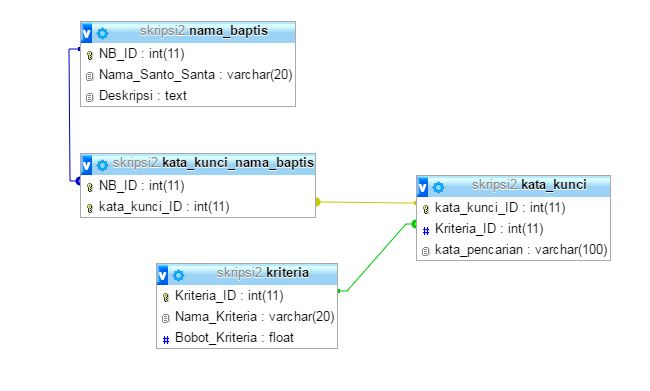
\includegraphics[scale=0.8]{Gambar/desainerdatabase.JPG}
			%\caption{Desain Database}
	%	\label{fig:db4}
	%\end{figure}
	

%\subsection{Bagian Tabel nama\_baptis}
%\label{sec:bagiantabelnb}

%Tabel ini digunakan untuk melihat nama baptis, beserta penjelasan detail dari nama baptis tersebut. %makna atau arti, tanggal pesta, nama lain, dan juga lambang dari nama baptis tersebut . 
	%Pada tabel nama\_baptis terdapat 3 kolom, yaitu:
	
	%\begin{itemize}
		%\item NB\_ID % (Gambar \ref{fig:db1})		
		
	%	\begin{itemize}
	%		\item Digunakan untuk memudahkan pengindeksan.
	%		\item Menggunakan jenis variabel int dengan panjang atau nilai 11.
	%		\item Menggunakan primary key (PK)\\
	%		NB\_ID menggunakan PK, karena PK merupakan kunci utama pada tabel database yang berfungsi sebagai kunci pengurutan data. Pada tabel hanya diperbolehkan memiliki satu PK.
		%	\item Menggunakan \textit{auto increment}\\
		%	NB\_ID menggunakan \textit{auto increment}, karena \textit{auto increment} merupakan tipe \textit{field} integer yang secara otomatis akan bertambah nilainya jika terjadi penambahan \textit{row} pada tabel di mana \textit{field} tersebut berada. Otomatis di sini artinya adalah pada saat memasukkan data baik melalui \textit{statement} INSERT maupun melalui mekanisme data akses lainnya, \textit{field} tersebut tidak perlu dimasukkan nilainya atau cukup diberi nilai NULL, maka MySQL akan menentukan sendiri nilai yang akan diberikan sebagai penambahan baris data tersebut. 
		%\end{itemize}
		
		%\item Nama\_Santo\_Santa %(Gambar \ref{fig:db3})
			
		%\begin{itemize}
		%	\item Digunakan untuk melihat nama santo-santa atau orang-orang kudus.
			%\item Menggunakan jenis variabel varchar dengan panjang atau nilai 20.
		%\end{itemize}
		
		%\item Deskripsi %(Gambar \ref{fig:db2})

%		\begin{itemize}
%			\item Digunakan untuk melihat penjelasan dari masing-masing santo-santa. Penjelasannya terdiri dari makna atau arti, nama lain santo-santa, lambang, dan tanggal pesta. 
	%		\item Menggunakan jenis variabel text.
		%\end{itemize}
%	\end{itemize}


%\subsection{Bagian Tabel kriteria}
%\label{sec:bagiantabelkriteria}

	%Tabel ini digunakan untuk melihat berbagai macam kriteria yang dipilih dan bobot kriteria. Pada tabel kriteria terdapat 3 kolom, yaitu:
	
%\begin{itemize}
%	\item Kriteria\_ID %(Gambar \ref{fig:db7})

	
%	\begin{itemize}
%		\item Digunakan untuk memudahkan pengindeksan.
%		\item Menggunakan jenis variabel int dengan panjang atau nilai 11.
%		\item Menggunakan primary key (PK)
		
	%		Kriteria\_ID menggunakan PK, karena PK merupakan kunci utama pada tabel database yang berfungsi sebagai kunci pengurutan data. Pada tabel hanya diperbolehkan memiliki satu PK.
		%\item Menggunakan \textit{auto increment}
		
		%Kriteria\_ID menggunakan \textit{auto increment}, karena \textit{auto increment} merupakan tipe \textit{field} integer yang secara otomatis akan bertambah nilainya jika terjadi penambahan \textit{row} pada tabel di mana \textit{field} tersebut berada. Otomatis di sini artinya adalah pada saat memasukkan data baik melalui \textit{statement} INSERT maupun melalui mekanisme data akses lainnya, \textit{field} tersebut tidak perlu dimasukkan nilainya atau cukup diberi nilai NULL, maka MySQL akan menentukan sendiri nilai yang akan diberikan sebagai penambahan baris data tersebut.
	%\end{itemize}
	
	%\item Nama\_Kriteria %(Gambar \ref{fig:db8})
	
	%\begin{itemize}
		%\item Digunakan untuk melihat kriteria, seperti arti Santo-Santa, deskripsi, tanggal lahir calon baptis, tanggal pembaptisan, profesi, lambang, serta pesta santo-santa.
		%\item Menggunakan jenis variabel varchar dengan panjang atau nilai 20.

%	\end{itemize}
%	\item Bobot\_Kriteria %(Gambar \ref{fig:db9})
	
	%\begin{itemize}
		%\item Digunakan untuk melihat bobot (W) yang sudah ditentukan untuk masing-masing kriteria.
		%\item Menggunakan jenis variabel float, karena mengandung pecahan.
	%	\end{itemize}
%\end{itemize}

%\subsection{Bagian Tabel Kata\_Kunci}
%\label{sec:bagiantabelkk}
%Tabel ini digunakan untuk melakukan pengelompokkan kata dan dapat yang dicari oleh \textit{user} . Pada tabel kata\_kunci terdapat 3 kolom, yaitu:

	
%	\begin{itemize}
	%	\item Kata\_kunci\_ID %(Gambar \ref{fig:db11})
		
		%	\begin{itemize}
		%\item Digunakan untuk memudahkan pengindeksan.
		%\item Menggunakan jenis variabel int dengan panjang atau nilai 11.
		%\item Menggunakan primary key (PK)
		
			%Kriteria\_ID menggunakan PK, karena PK merupakan kunci utama pada tabel database yang berfungsi sebagai kunci pengurutan data. Pada tabel hanya diperbolehkan memiliki satu PK.
		%\item Menggunakan \textit{auto increment}
		
		%Kriteria\_ID menggunakan \textit{auto increment}, karena \textit{auto increment} merupakan tipe \textit{field} integer yang secara otomatis akan bertambah nilainya jika terjadi penambahan \textit{row} pada tabel di mana \textit{field} tersebut berada. Otomatis di sini artinya adalah pada saat memasukkan data baik melalui \textit{statement} INSERT maupun melalui mekanisme data akses lainnya, \textit{field} tersebut tidak perlu dimasukkan nilainya atau cukup diberi nilai NULL, maka MySQL akan menentukan sendiri nilai yang akan diberikan sebagai penambahan baris data tersebut.
	%\end{itemize}
		
		%\item Kriteria\_ID %(Gambar \ref{fig:db12})
		
		%\begin{itemize}
		%	\item Digunakan untuk mengambil data dari tabel kriteria.
		%	\item Merupakan foreign key (fk) dari tabel kriteria.
		%	\item Menggunakan jenis variabel int dengan panjang atau nilai 11.
		%\end{itemize}
		
		%\item Kata\_pencarian %(Gambar \ref{fig:db13})
		
%		\begin{itemize}
%			\item Digunakan untuk mencari kata yang dimasukkan oleh \textit{user}.
%			\item Menggunakan jenis variabel varchar dengan panjang atau nilai 100.
%			\item Berisi kata yang sudah dikelompokkan agar memudahkan dalam pencarian. Sebagai contoh adalah kata agung dan besar, kata-kata tersebut sudah dijadikan satu kesatuan atau dikelompokkan, agar jika \textit{user} mencari kata ``besar'' yang tidak ada pada suatu deskripsi pada tabel nama\_baptis, akan tetap keluar sebagai hasil \textit{output}. Hasil \textit{output} yang akan keluar untuk kata ``besar'' adalah deskripsi yang mengandung kata ``agung'', karena kata ``besar'' sudah tersimpan dan sudah dikelompokkan dengan kata ``agung'' pada kata\_pencarian.
			
	%	\end{itemize}
	%\end{itemize}
	
	%\subsection{Bagian Tabel Kata\_Kunci\_Nama\_Baptis}
%\label{sec:bagiantabelkknb}
%Tabel ini digunakan untuk membuat tabel kata\_kunci dengan tabel nama\_baptis menjadi satu, sehingga sistem dapat mengetahui yang \textit{user} \textit{input} atau masukkan pada kata\_pencarian dan mencocokan kata yang dimasukkan \textit{user} tersebut dengan nama\_baptis yang ada pada tabel nama\_baptis. Dengan demikian, hasil alternatif akan keluar sesuai dengan yang diinginkan oleh \textit{user}. Pada tabel Kata\_Kunci\_Nama\_Baptis terdapat 2 kolom, yaitu:

%	\begin{itemize}
	%	\item NB\_ID %(Gambar \ref{fig:db16})
		
	
%		\begin{itemize}
%		\item Merupakan foreign key (fk) dari tabel nama\_baptis
%		\item Menggunakan jenis variabel int dengan panjang atau nilai 11.
%		\item Digunakan untuk mengambil data dari tabel nama\_baptis
%		\end{itemize}
		
	%	\item Kata\_Kunci\_ID %(Gambar \ref{fig:db17})
		
%		\begin{itemize}
%		\item Merupakan foreign key (fk) dari tabel kata\_kunci
%		\item Menggunakan jenis variabel int dengan panjang atau nilai 11.
%		\item Digunakan untuk mengambil data dari tabel kata\_kunci
%		\end{itemize}
%\end{itemize}

	%Dari hasil analisis database sebelumnya, dapat disimpulkan bahwa \textit{user} dapat memasukkan \textit{input} berupa kriteria, seperti tanggal lahir calon baptis, tanggal pembaptisan, arti, lambang, profesi dan sebagainya (\textit{input} dapat lebih dari 1). Setelah \textit{user} memasukkan \textit{input} tersebut, maka database akan mencari pada tabel kata\_kunci. Setelah kata yang dicari tersebut sudah ditemukan pada tabel kata\_kunci, kemudian tabel kata\_kunci di JOIN dengan tabel kata\_kunci\_nama\_baptis, untuk mendapatkan NB\_ID dan kriteria. NB\_ID didapatkan untuk mencocokkan kata yang dicari oleh \textit{user} dengan nama baptis yang ada pada database (tabel nama\_baptis), sedangkan kriteria didapatkan agar database dapat mengetahui \textit{user} memasukkan \textit{input} berdasarkan kriteria jenis apa. Setelah mendapatkan kriteria dan NB\_ID, kemudian kedua tabel yang sudah di JOIN harus di JOIN dengan tabel nama\_baptis, agar mendapatkan nama baptis dan deskripsi yang diinginkan oleh \textit{user}.
	
	%\textit{Syntax} JOIN dalam MySQL digunakan untuk menggabungkan beberapa tabel, untuk mendapatkan data \cite{sqljoin}. Menggunakan \textit{Syntax} JOIN karena beberapa tabel dapat digabungkan, sehingga dapat dihasilkan sekumpulan \textit{output} tunggal, dan JOIN menghubungkan record-record yang benar di setiap tabel.
	
	%Hasil pada database merupakan data mentah, dengan kata lain masih belum dapat dikatakan hasil akhir. Data mentah tersebut harus diolah kembali agar mendapatkan hasil yang benar-benar dicari oleh \textit{user}, yaitu dengan menggunakan perhitungan pada metode SAW, dimana membutuhkan bobot pada setiap kriterianya.
	
	
	%akan dilakukan pencarian dengan cara mencocokkan kata yang dicari oleh \textit{user}, yang sudah ada pada tabel kata\_kunci. Setelah menemukan kata yang dicari tersebut pada tabel kata\_kunci, maka tabel tersebut akan di JOIN dengan tabel kata\_kunci\_nama\_baptis. Tabel kata\_kunci\_nama\_baptis akan mencocokkan kata yang dicari oleh \textit{user} dengan tabel nama\_baptis, apakah  Selain menemukan kata yang dicari pada tabel kata\_kunci, sistem juga akan mendapatkan, berdasarkan kriteria apa, user mencari kata tersebut. Kemudian setelah kata yang dicari ditemukan, maka akan di JOIN lagi dengan tabel kriteria untuk mendapatkan bobotnya. Dengan demikian, akan dikeluarkan hasil berupa nama baptis yang sesuai dengan yang diinginkan atau yang dicari oleh \textit{user}.
	
%\subsection{Contoh Kasus SPK Pemilihan Nama Baptis (\textit{user} hanya memasukkan atau memilih 1 kriteria)}
%\label{sec:contohkasus}
	
	%Pada pemilihan nama baptis, \textit{user} akan memasukkan 1 kriteria. Salah satu contoh kriteria adalah arti nama santo-santa. Berikut adalah contoh kode untuk melakukan pencarian daftar nama baptis yang mengandung arti kata ``mulia''.
	
	
	%\begin{lstlisting}
		%select nama_baptis.Nama_Santo_Santa, nama_baptis.deskripsi FROM `nama_baptis` 
		%INNER JOIN kata_kunci_nama_baptis ON nama_baptis.NB_ID=kata_kunci_nama_baptis.NB_ID
		%INNER JOIN kata_kunci ON kata_kunci_nama_baptis.kata_kunci_ID=kata_kunci_ID 
		%INNER JOIN kriteria ON kata_kunci.kriteria_ID=kriteria.kriteria_ID
		%WHERE kata_kunci.kata_pencarian like ``\%mulia\%'' AND kriteria.kriteria_ID = 1
	%\end{lstlisting}
	
	%\begin{figure}[htbp]
	%	\centering
	%		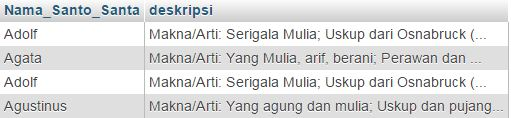
\includegraphics[scale=0.7]{Gambar/contohkasus2.JPG}
	%		\caption{\textit{Hasil Output}}
	%	\label{fig:contohkasus2}
	%\end{figure}
	
  %Hasil \textit{output} yang akan dikeluarkan adalah nama baptis dan deskripsi yang masih mentah (Gambar \ref{fig:contohkasus2}). Pada gambar tersebut, terdapat 4 hasil nama, yang di dalamnya mencakup kata ``mulia''. Keempat nama tersebut belum dapat dikatakan sebagai alternatif, karena pada metode SAW, perlu adanya pembobotan pada masing-masing kriteria, yang menjadikan nama tersebut dapat dikatakan sebagai alternatif. Berikut adalah contoh kode untuk melakukan pencarian daftar nama baptis yang mengandung arti kata ``mulia'' beserta bobotnya pada masing-masing kriteria.

%	, maka akan muncul seperti pada gambar \ref{fig:contohkasus4}, yang mana terdapat bobot pada masing-masing kata yang dicari oleh \textit{user}, berdasarkan kriteria 1, yaitu arti santo-santa, dengan bobot 0.4.
		
%	\begin{lstlisting}
%		select nama_baptis.Nama_Santo_Santa, nama_baptis.deskripsi kriteria.bobot_kriteria FROM `nama_baptis` 
%		INNER JOIN kata_kunci_nama_baptis ON nama_baptis.NB_ID=kata_kunci_nama_baptis.NB_ID
%		INNER JOIN kata_kunci ON kata_kunci_nama_baptis.kata_kunci_ID=kata_kunci_ID 
%		INNER JOIN kriteria ON kata_kunci.kriteria_ID=kriteria.kriteria_ID
%		WHERE kata_kunci.kata_pencarian like ``\%mulia\%'' AND kriteria.kriteria_ID = 1
%	\end{lstlisting}
	

%	\begin{figure}[htbp]
%		\centering
%			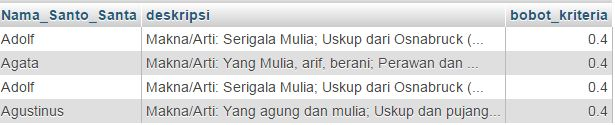
\includegraphics[scale=0.7]{Gambar/contohkasus4.JPG}
%			\caption{\textit{Hasil Output}}
%		\label{fig:contohkasus4}
%	\end{figure}
	
	% Hasil \textit{output} yang akan dikeluarkan adalah nama baptis, deskripsi yang masih mentah dan bobot dari masing-masing kriteria (Gambar\ref{fig:contohkasus4}). Pada gambar tersebut, terdapat 4 hasil nama, yang di dalamnya mencakup kata ``mulia''. Selain terdapat kata ``mulia'', juga terdapat bobot pada tabel tersebut. Keempat nama tersebut belum dapat dikatakan sebagai alternatif, karena pada metode SAW, perlu adanya pembobotan pada masing-masing kriteria, yang menjadikan nama tersebut dapat dikatakan sebagai alternatif.
	
	
	%\subsection{Contoh Kasus SPK Pemilihan Nama Baptis (\textit{user} memasukkan atau memilih lebih dari 1 kriteria)}
%\label{sec:contohkasus1}
	
	%Pada pemilihan nama baptis, \textit{user} akan memasukkan beberapa kriteria. Salah satu contoh kriteria adalah arti nama santo-santa, lambang dan tanggal lahir. Berikut adalah contoh kode untuk melakukan pencarian daftar nama baptis yang mengandung arti kata ``mulia'', lambang ``puteri'' dan tanggal lahir ``juni''.
	
	
	%\begin{lstlisting}
		%select nama_baptis.Nama_Santo_Santa, nama_baptis.deskripsi kriteria.bobot_kriteria FROM `nama_baptis` 
		%INNER JOIN kata_kunci_nama_baptis ON nama_baptis.NB_ID=kata_kunci_nama_baptis.NB_ID
		%INNER JOIN kata_kunci ON kata_kunci_nama_baptis.kata_kunci_ID=kata_kunci.kata_kunci_ID 
		%INNER JOIN kriteria ON kata_kunci.kriteria_ID=kriteria.kriteria_ID
		%WHERE (kata_kunci.kata_pencarian like ``\%mulia\%'' AND kriteria.kriteria_ID = 1) OR (kata_kunci.kata_pencarian like ``\%juni\%'' AND kriteria.kriteria_ID = 3) OR (kata_kunci.kata_pencarian like ``\%puteri\%'' AND kriteria.kriteria_ID = 6)
	%\end{lstlisting}
	
	
%\begin{figure}[htbp]
%		\centering
%			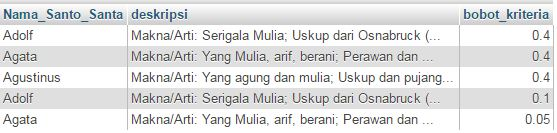
\includegraphics[scale=0.7]{Gambar/contohkasus7.JPG}
%			\caption{\textit{Hasil Output}}
%		\label{fig:contohkasus7}
%	\end{figure}
	
	
	%Hasil \textit{output} yang akan dikeluarkan adalah nama baptis, deskripsi dan bobot dari masing-masing kriteria yang masih mentah (Gambar \ref{fig:contohkasus7}). Yang dimaksud mentah di sini adalah belum dapat dikatakan sebagai alternatif. Pada gambar tersebut, terdapat 5 hasil nama, yang di dalamnya mencakup kata ``mulia''. Yang mencakup kata ``mulia'' terhitung 1 sampai 2 kali muncul. Selain terdapat kata ``mulia'', juga terdapat kata ``puteri'' dan ``juni''. Selain terdapat nama dan deskripsi, juga terdapat bobot pada tabel tersebut. Kelima nama tersebut belum dapat dikatakan sebagai alternatif, karena pada metode SAW, perlu adanya pembobotan pada masing-masing kriteria, yang menjadikan nama tersebut dapat dikatakan sebagai alternatif. Bobot pada masing-masing kriteria berbeda-beda. Bobot pada kriteria arti adalah 0.4, bobot pada kriteria lambang adalah 0.05, dan bobot pada kriteria tanggal lahir adalah 0.1.
	
	
  %Hasil \textit{output} yang akan dikeluarkan sebagai alternatif untuk \textit{user} dapat memilih nama baptis yang cocok adalah dapat dilihat pada gambar \ref{fig:contohkasus7}. Pada gambar tersebut, terdapat 5 hasil nama, yang terhitung terdapat 1 atau 2 kali muncul, yang di dalamnya mencakup kata ``mulia'', ``puteri'', dan ``juni''. Terdapat bobot yang berbeda pada masing-masing nama, yang mana mengacu pada bobot kriteria. Hasil dengan nama Adolf mempunyai 2 data, yang mana di dalamnya mencakup kata ``mulia'', dengan bobot 0.4, dan ``juni'', dengan bobot 0.1. Hasil dengan nama Agata mempunyai 2 data, yang mana di dalamnya mencakup kata ``mulia'', dengan bobot 0.4, dan ``puteri'', dengan bobot 0.05. Dan hasil dengan nama Agustinus hanya mempunyai 1 data, yang mana di dalamnya mencakup kata ``mulia'', dengan bobot 0.4.
	%Keempat nama tersebut belum dapat dikatakan sebagai alternatif, karena pada metode SAW, perlu adanya pembobotan pada masing-masing kriteria, yang menjadikan nama tersebut dapat dikatakan sebagai alternatif. Jika memasukkan \textit{statement} seperti pada gambar \ref{fig:contohkasus3}, maka akan muncul seperti pada gambar \ref{fig:contohkasus4}, yang mana terdapat bobot pada masing-masing kata yang dicari oleh \textit{user}, berdasarkan kriteria 1, yaitu arti santo-santa, dengan bobot 0.4.
	
\section{Analisis \textit{Perangkat Lunak}}
\label{sec:analisisusecase}
\subsection{Diagram \textit{Use Case}}
\label{sec:diagramusecase}
	Diagram \textit{use case} pada perangkat lunak yang akan dibangun hanya mengandung 2 aktor, yaitu calon baptis sebagai \textit{user} dan admin.  Diagram \textit{use case} dapat dilihat pada Gambar  \ref{fig:usecase}.

	\begin{figure}[htbp]
		\centering
			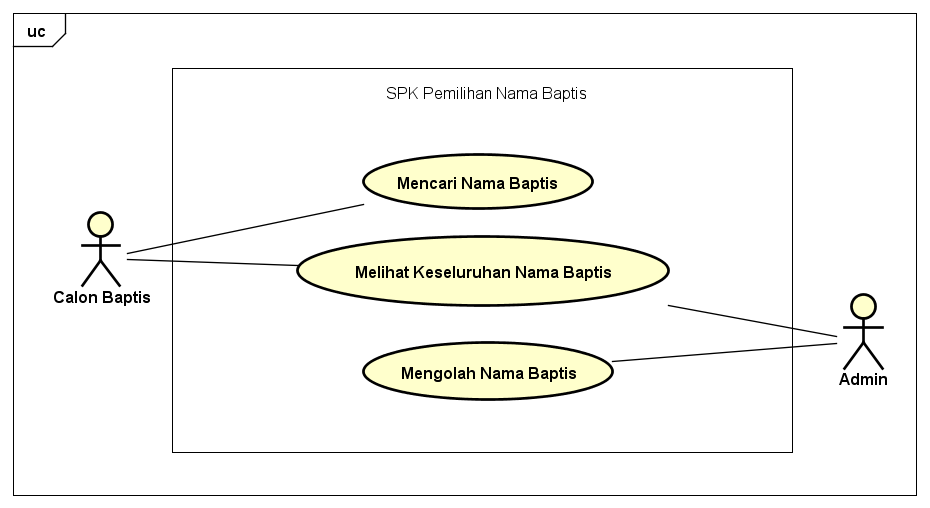
\includegraphics[scale=0.7]{Gambar/usecase.PNG}
			\caption{\textit{Diagram \textit{Use Case} SPK Pemilihan Nama Baptis}}
		\label{fig:usecase}
	\end{figure}

	Berdasarkan hasil analisis  pada subbab analisis kuesioner, dibentuk 3 \textit{use case} dengan 2 aktor, antara lain:
	\begin{itemize}
			\item \textbf{\textit{User}}
				\begin{itemize}
					\item \textbf{Mencari Nama Baptis}

					Calon baptis dapat melihat dan atau memilih kategori apa saja yang dapat digunakan sebagai patokan untuk memilih nama baptis yang cocok, memasukkan \textit{input} seperti kata kunci, dan melihat hasil \textit{output} berupa nama baptis dan deskripsinya. Kategori yang dapat dijadikan patokan atau acuan adalah tanggal lahir calon baptis, tanggal pesta santo-santa, lambang santo-santa, arti nama dari santo-santa, tanggal pembaptisan, deskripsi dari santo-santa, dan profesi dari santo-santa.
					%\item \textbf{Memasukkan \textit{Input}}

					%Calon baptis dapat memasukkan \textit{Input} seperti kata kunci untuk mencari nama baptis yang mereka inginkan.
					%\item \textbf{Melihat Hasil \textit{Output}}

					%Calon baptis dapat melihat hasil \textit{Output} yang dijadikan sebagai alternatif pemilihan nama baptis. Terlebih dahulu calon baptis memasukkan kata kunci dan juga kategori yang diinginkan untuk dijadikan pedoman, agar alternatif dapat dihasilkan dan calon baptis tersebut dapat memilih nama baptis yang diinginkan.
					\item \textbf{Melihat Keseluruhan Nama Baptis}

					Calon baptis atau pengguna umum dapat melihat keseluruhan nama baptis beserta deskripsi di dalamnya.
				\end{itemize}
			\item \textbf{Admin}
				\begin{itemize}
				\item \textbf{Melihat Keseluruhan Nama Baptis}

					Admin dapat melihat keseluruhan nama baptis beserta deskripsi di dalamnya.
					
					\item \textbf{Mengolah Nama Baptis}

					Admin dapat melakukan \textit{update} atau memperbaharui nama baptis, menambahkan nama baptis, dan menghapus nama baptis. Admin dapat memperbaharui nama baptis, serta informasi atau deskripsi yang ada di dalamnya, seperti arti, lambang, profesi dari santo-santa tersebut dan lain sebagainya. Selain dapat memperbaharui, admin juga dapat menambahkan dan menghapus nama baptis serta informasi yang ada di dalamnya.
					%\item \textbf{Menambahkan Nama Baptis}

					%Admin dapat menambahkan nama baptis, dan juga deskripsi atau informasi di dalamnya.
					%\item \textbf{Menghapus Nama Baptis}

					%Admin dapat menghapus nama baptis yang sekiranya tidak terlalu lengkap informasinya.
				\end{itemize}
	\end{itemize}
	
\textbf{Skenario \textit{Use Case}}
\label{sec:skenariousecase}
\begin{enumerate}
\item \textit{User}


                       \begin{enumerate}
                        \item Mencari Nama Baptis
                                \begin{itemize}
                                        \item Nama: Mencari Nama Baptis
                                        \item Aktor: Calon Baptis
                                        \item Deskripsi: Memilih kategori, memasukkan \textit{input}, dan dapat melihat hasil \textit{output} yang sesuai dengan yang dinginkan oleh calon baptis.
                                        \item Kondisi awal: Calon baptis telah membuka web pemilihan nama baptis dan telah memilih kategori, serta memasukkan \textit{input} berupa kata kunci. %msh bingung
                                        \item Kondisi akhir: Web akan menampilkan nama baptis yang dapat dipilih oleh calon baptis.%msh bingung
                                        \item Skenario utama:														
				
				
				\begin{table}[H]
	\centering
	\caption{Tabel Skenario Mencari Nama Baptis}
		\begin{tabular}{| c | p{6cm} |p{6cm} |} \hline
     No  & Aksi & Reaksi Sistem\\ \hline 
		1 & Calon baptis memilih kategori yang telah disediakan, 
		seperti tanggal lahir, profesi, arti dan lain sebagainya. %beserta
		%kata kunci agar memudahkan calon baptis memilih alternatif yang telah di keluarkan. 
		&  Sistem mendapatkan data dari calon baptis berupa kategori yang dipilih.\\ \hline 
		2 & Calon baptis memasukkan \textit{input} berupa kata kunci. & Sistem mendapatkan data dari calon baptis berupa kata kunci dan menampilkan hasil pencarian berdasarkan kata kunci. \\ \hline
		
		3 & Calon baptis melihat dan memilih hasil \textit{output} berupa alternatif nama baptis. & Tidak ada reaksi sistem.\\ \hline
				\end{tabular}
	\label{table:skenario1}
\end{table}
				
				
		                                \end{itemize}
																	 \item Melihat Keseluruhan Nama Baptis

                         \begin{itemize}
                                        \item Nama: Melihat Keseluruhan Nama Baptis
                                        \item Aktor: Calon Baptis atau pengguna umum
                                        \item Deskripsi: Melihat nama baptis dan informasinya
                                        \item Kondisi awal: calon baptis atau pengguna umum telah membuka web pemilihan nama baptis  %msh bingung
                                        \item Kondisi akhir: calon baptis atau pengguna umum dapat melihat nama baptis serta informasinya %msh bingung
                                        \item Skenario utama:														
				
				\begin{table}[H]
	\centering
	\caption{Tabel Skenario Melihat Keseluruhan Nama Baptis (calon baptis/pengguna umum)}
		\begin{tabular}{ | c | p{5cm} |p{5cm} |} \hline
     No  & Aksi & Reaksi Sistem\\ \hline 
				1 & Calon baptis atau pengguna umum memilih menu semua nama baptis.% agar memudahkan calon baptis memilih alternatif yang telah di keluarkan. 
				&  Sistem menampilkan seluruh nama baptis.\\ \hline
		
						\end{tabular}
	\label{table:skenario2}
\end{table}
				
				
				                       
                                \end{itemize}
																\end{enumerate}
																\item Admin
																\begin{enumerate}
																\item Melihat Keseluruhan Nama Baptis
									
                         \begin{itemize}
                                        \item Nama: Melihat keseluruhan nama baptis
                                        \item Aktor: Admin
                                        \item Deskripsi: Melihat nama baptis dan informasinya
                                        \item Kondisi awal: Admin telah membuka web pemilihan nama baptis  %msh bingung
                                        \item Kondisi akhir: Admin dapat melihat nama baptis serta informasinya %msh bingung
                                        \item Skenario utama:														
				
				\begin{table}[H]
	\centering
	\caption{Tabel Skenario Melihat Keseluruhan Nama Baptis (admin)}
		\begin{tabular}{ | c | p{5cm} |p{5cm} |} \hline
     No  & Aksi & Reaksi Sistem\\ \hline 
				1 & Admin memilih menu semua nama baptis.% agar memudahkan calon baptis memilih alternatif yang telah di keluarkan. 
				&  Sistem menampilkan seluruh nama baptis.\\ \hline
		
						\end{tabular}
	\label{table:skenario3}
\end{table}
				
				
																
																       \end{itemize}
																
                                \item Mengolah Nama Baptis
\begin{itemize}
\item Memperbaharui Nama Baptis
\begin{itemize}
                                        \item Nama: Memperbaharui Nama Baptis
                                        \item Aktor: Admin
                                        \item Deskripsi: Dapat memperbaharui data yang sudah ada sebelumnya, menambahkan data baru, dan menghapus data yang tidak terpakai.
                                        \item Kondisi awal: Data lama sudah terdapat pada sistem. %msh bingung
                                        \item Kondisi akhir: Data lama telah diperbaharui dengan data baru. %msh bingung
            
																				
																				\item Skenario utama:														
			\begin{table}[H]
	\centering
	\caption{Tabel Skenario Memperbaharui Nama Baptis}
		\begin{tabular}{ | c | p{5cm} |p{5cm} |} \hline
     No  & Aksi & Reaksi Sistem\\ \hline 
				1 & Admin mengubah nama baptis dan informasinya.% agar memudahkan calon baptis memilih alternatif yang telah di keluarkan. 
				&  Sistem akan mengubah nama baptis dan informasi lama menjadi sesuai dengan \textit{input} admin.\\ \hline
		
						\end{tabular}
	\label{table:skenario4}
\end{table}
			
			

                                \end{itemize}
		\item Menambahkan Nama Baptis

                                \begin{itemize}
                                        \item Nama: Menambahkan nama baptis
                                        \item Aktor: Admin
                                        \item Deskripsi: Dapat menambahkan data baru
                                        \item Kondisi awal: data belum ada pada sistem %msh bingung
                                        \item Kondisi akhir: data baru sudah ditambahkan dan akan ditampilkan%msh bingung
                                        \item Skenario utama:														
				
				
				\begin{table}[H]
	\centering
	\caption{Tabel Skenario Menambahkan Nama Baptis}
		\begin{tabular}{ | c | p{5cm} |p{5cm} |} \hline
     No  & Aksi & Reaksi Sistem\\ \hline 
				1 & Admin menambahkan nama baptis beserta informasinya.% agar memudahkan calon baptis memilih alternatif yang telah di keluarkan. 
				&  Sistem akan menambahkan nama baptis beserta informasinya.\\ \hline
		
						\end{tabular}
	\label{table:skenario5}
\end{table}
				
				

                                \end{itemize}
																\item Menghapus Nama Baptis

                                \begin{itemize}
                                        \item Nama: Menghapus nama baptis
                                        \item Aktor: Admin
                                        \item Deskripsi: Dapat menghapus data yang terlihat tidak begitu lengkap atau tidak begitu terpakai.
                                        \item Kondisi awal: sebelumnya terdapat data pada sistem %msh bingung
                                        \item Kondisi akhir: data telah dihapus dan tidak akan muncul di tampilan%msh bingung
                                        \item Skenario utama:														
				
				\begin{table}[H]
	\centering
	\caption{Tabel Skenario Menghapus Nama Baptis}
		\begin{tabular}{ | c | p{5cm} |p{5cm} |} \hline
     No  & Aksi & Reaksi Sistem\\ \hline 
				1 & Admin menghapus nama baptis dan informasinya.% agar memudahkan calon baptis memilih alternatif yang telah di keluarkan. 
				&  Sistem akan menghapus nama baptis dan informasinya yang telah dipilih oleh admin.\\ \hline
		
						\end{tabular}
	\label{table:skenario6}
\end{table}
				
		
\end{itemize}
\end{itemize}
 \end{enumerate}
 \end{enumerate}%Berdasarkan hasil analisis pada subbab \ref{sec:analisiskuesioner}, 
%\subsection{Bagian Menambahkan Rute}
%\label{sec:menambahkanrute}
%Bagian ini terletak di baris 97-117 dari ``handle.php'' (kode \ref{lst:handle.php}). Bagian ini akan dieksekusi jika terdapat parameter ``\texttt{mode=addtrack}'' pada permintaan POST. Bagian ini berfungsi untuk menambahkan sebuah rute jalan yang dapat ditempuh oleh kendaraan umum tertentu (contoh: angkot).

%Bagian ini diawali dengan memeriksa apakah pengguna memiliki hak akses untuk menambahkan rute atau tidak (baris 98). Lalu memeriksa apakah pengguna mengirimkan data \textit{trackid}, \textit{trackname}, \textit{tracktype}, \textit{penalty}, dan \textit{internalinfo} pada permintaan atau tidak (baris 99-103). Setelah itu, program akan mengecek apakah rute jalan yang ingin ditambahkan pengguna sudah ada atau belum di \textit{database} (106-114). Bila rute jalan belum ada, maka rute jalan akan ditambahkan ke dalam \textit{database} (baris 109) dan \textit{server} akan mengirimkan pesan dalam format JSON (baris 116) sebagai penanda bahwa pengguna berhasil menambahkan rute jalan.

%\subsection{Bagian Mengubah Rute}
%\label{sec:mengubahrute}
%Bagian ini terletak di baris 117-146 dari ``handle.php'' (kode \ref{lst:handle.php}). Bagian ini akan dieksekusi jika terdapat parameter ``\texttt{mode=updatetrack}'' pada permintaan POST. Bagian ini berfungsi untuk mengubah data sebuah rute jalan yang dapat ditempuh oleh kendaraan umum tertentu (contoh: angkot).

%Bagian ini diawali dengan memeriksa apakah pengguna memiliki hak akses untuk mengubah rute atau tidak (baris 118). Lalu memeriksa apakah pengguna mengirimkan data \textit{trackid}, \textit{newtrackid}, \textit{trackname}, \textit{tracktype}, \textit{penalty}, \textit{pathloop}, \textit{transfernodes}  dan \textit{internalinfo} pada permintaan atau tidak (baris 119-126). Setelah itu, \textit{server} akan mengecek apakah rute yang ingin diubah pengguna sudah memenuhi aturan (\textit{trackid} harus sama dengan \textit{newtrackid}) atau tidak (129-143). Bila rute yang ingin diubah maka \textit{server} akan mengirimkan pesan dalam format JSON sebagai penanda bahwa pengguna berhasil mengubah rute rute jalan.

%\subsection{Bagian Melihat Daftar Rute}
%\label{sec:melihatdaftarrute}
%Bagian ini terletak di baris 146-172 dari ``handle.php'' (kode \ref{lst:handle.php}). Bagian ini akan dieksekusi jika terdapat parameter ``\texttt{mode=listtracks}'' pada permintaan POST. Bagian ini berfungsi untuk memberikan daftar rute jalan yang terdapat dalam \textit{database} sistem KIRI.

%Bagian ini diawali dengan memeriksa apakah pengguna memiliki hak akses terhadap rute jalan atau tidak (baris 147). Setelah itu program akan mengambil data daftar rute jalan yang terdapat pada \textit{database} sistem KIRI (baris 149-154). Lalu program juga akan mengambil data daftar tipe rute jalan dari \textit{database} (baris 156-161). Data-data yang diperoleh program (rute jalan dan tipe rute jalan) akan diubah formatnya menjadi sebuah data JSON (baris 164-168). Terakhir, program akan mengirimkan data dalam format JSON tersebut ke pengguna (baris 171).

%\subsection{Bagian Melihat Informasi Rute secara Detail}
%\label{sec:melihatdaftarrutedetail}
%Bagian ini terletak di baris 172-200 dari ``handle.php'' (kode \ref{lst:handle.php}). Bagian ini akan dieksekusi jika terdapat parameter ``\texttt{mode=getdetailstrack}'' pada permintaan POST. Bagian ini berfungsi untuk memberikan informasi detail tentang suatu rute jalan.

%Bagian ini diawali dengan memeriksa apakah pengguna memiliki hak akses terhadap rute jalan atau tidak (baris 173). Lalu program akan memeriksa apakah pengguna memberikan \textit{trackid} pada permintaan atau tidak (baris 174). Selanjutnya program akan mengambil data dari \textit{database} sistem KIRI (baris 177-184). Data yang diperoleh dari \textit{database} tersebut akan diubah formatnya ke dalam format JSON (baris 186-196). Terakhir, program akan mengirimkan data dalam format JSON tersebut ke pengguna (baris 199).

%\subsection{Bagian Menghapus Data Geografis suatu Rute}
%\label{sec:hapusdatageografis}
%Bagian ini terletak di baris 200-209 dari ``handle.php'' (kode \ref{lst:handle.php}). Bagian ini akan dieksekusi jika terdapat parameter ``\texttt{mode=cleargeodata}'' pada permintaan POST. Bagian ini berfungsi untuk menghapus data geografis suatu rute jalan yang terdapat dalam \textit{database} sistem KIRI.

%Bagian ini diawali dengan memeriksa apakah pengguna memiliki hak akses terhadap rute jalan atau tidak (baris 201). Lalu program akan memeriksa apakah pengguna memberikan \textit{trackid} pada permintaan atau tidak (baris 202). Program akan langsung menghapus data geografis rute jalan sesuai dengan \textit{trackid} permintaan pengguna jika \textit{trackid} tersebut terdapat dalam \textit{database} sistem KIRI (baris 204-205). Terakhir, program akan mengirimkan pesan keberhasilan dalam format JSON kepada pengguna (baris 208).

%\subsection{Bagian Impor Data KML}
%\label{sec:imporkml}
%Bagian ini terletak di baris 209-246 dari ``handle.php'' (kode \ref{lst:handle.php}). Bagian ini akan dieksekusi jika terdapat parameter ``\texttt{mode=importkml}'' pada permintaan POST. Bagian ini berfungsi untuk menambahkan data geografis suatu rute dimana data yang ditambahkan berasal dari sebuah \textit{file} dengan format KML (\textit{Keyhole Markup Language}). KML adalah format \textit{file} yang digunakan untuk menampilkan data geografis dalam aplikasi pemetaan\cite{kml}. 

%Bagian ini diawali dengan memeriksa apakah pengguna memiliki hak akses terhadap rute jalan atau tidak (baris 210). Lalu program akan memeriksa apakah pengguna memberikan \textit{trackid} pada permintaan atau tidak (baris 211). Selanjutnya program akan memeriksa apakah \textit{file} pengguna memberikan \textit{file} dengan format sesuai atau tidak (baris 213-218). Pada baris 219-228 program akan mengambil data LineString yang terdapat pada \textit{file} dengan menggunakan teknik \textit{regular expression} (baris 224, referensi subbab \ref{sec:regex}). Baris 231-239 program akan membangun data LineString yang semula dalam format KML menjadi format WKT (subbab \ref{sec:wktformat}). Program akan menambahkan data LineString dalam WKT tersebut ke dalam \textit{database} sesuai dengan \textit{trackid} yang diberikan pengguna (baris 241-243). Terakhir, program akan mengirimkan pesan dalam format JSON sebagai penanda bahwa pengguna berhasil melakukan import data KML (baris 245).

%\subsection{Bagian Menghapus Rute}
%\label{sec:hapusrute}
%Bagian ini terletak di baris 246-261 dari ``handle.php'' (kode \ref{lst:handle.php}). Bagian ini akan dieksekusi jika terdapat parameter ``\texttt{mode=deletetrack}'' pada permintaan POST. Bagian ini berfungsi untuk menghapus suatu rute jalan yang terdapat dalam sistem KIRI.

%Bagian ini diawali dengan memeriksa apakah pengguna memiliki hak akses terhadap rute jalan atau tidak (baris 247). Lalu program akan memeriksa apakah pengguna memberikan \textit{trackid} pada permintaan atau tidak (baris 248). Program akan memeriksa apakah terdapat {trackid} yang sesuai dengan {trackid} yang ada pada \textit{database} KIRI (baris 250-259). Bila terdapat \textit{trackid} yang sesuai, maka program akan menghapus rute jalan tersebut. Terakhir, program akan mengirimkan pesan keberhasilan dalam format JSON kepada pengguna (baris 260).

%\subsection{Bagian Melihat Daftar API \textit{Keys}}
%\label{sec:lihatapikeys}
%Bagian ini terletak di baris 261-279 dari ``handle.php'' (kode \ref{lst:handle.php}). Bagian ini akan dieksekusi jika terdapat parameter ``\texttt{mode=listapikeys}'' pada permintaan POST. Bagian ini berfungsi untuk memberikan daftar API \textit{keys} yang terdapat dalam database sistem KIRI.

%Bagian ini diawali dengan memeriksa apakah pengguna memiliki hak akses terhadap penggunaan API atau tidak (baris 262). Setelah itu program akan mengambil data daftar API \textit{keys} yang terdapat pada \textit{database} sistem KIRI (baris 264-269). Data-data yang diperoleh program akan diubah formatnya menjadi sebuah data JSON (baris 272-275). Terakhir, program akan mengirimkan data dalam format JSON tersebut ke pengguna (baris 278).

%\subsection{Bagian Menambahkan API \textit{Key}}
%\label{sec:tambahapikey}
%Bagian ini terletak di baris 279-299 dari ``handle.php'' (kode \ref{lst:handle.php}). Bagian ini akan dieksekusi jika terdapat parameter ``\texttt{mode=addapikey}'' pada permintaan POST. Bagian ini berfungsi untuk menambahkan sebuah data API \textit{key} ke dalam sistem KIRI.

%Bagian ini diawali dengan memeriksa apakah pengguna memiliki hak akses terhadap API \textit{keys} atau tidak (baris 280). Lalu memeriksa apakah pengguna mengirimkan data \textit{domainfilter} dan \textit{description} pada permintaan atau tidak (baris 281-282). Setelah itu, program akan membangun sebuah API key secara acak (baris 283). Program akan menambahkan data API \textit{key} sesuai dengan data yang dikirimkan pengguna ke dalam \textit{database} KIRI (baris 286) dan mencatat proses penambahan tersebut ke dalam \textit{database} (baris 289). Terakhir, program akan membangun sebuah pesan keberhasilan dalam format JSON (baris 292-295) dan mengirimkan pesan tersebut kepada pengguna (baris 298).

%\subsection{Bagian Mengubah API \textit{Key}}
%\label{sec:ubahapikey}
%Bagian ini terletak di baris 299-317 dari ``handle.php'' (kode \ref{lst:handle.php}). Bagian ini akan dieksekusi jika terdapat parameter ``\texttt{mode=updateapikey}'' pada permintaan POST. Bagian ini berfungsi untuk mengubah data sebuah API \textit{key} pada \textit{database} sistem KIRI.

%Bagian ini diawali dengan memeriksa apakah pengguna memiliki hak akses terhadap API \textit{keys} atau tidak (baris 300). Lalu memeriksa apakah pengguna mengirimkan data \textit{apikey}, \textit{domainfilter}, dan \textit{description} pada permintaan atau tidak (baris 301-303). Setelah itu, program akan memeriksa apakah pengguna yang bersangkutan adalah pemilik API \textit{key} yang ingin diubah atau bukan (baris 305-311). Lalu program mengubah data API \textit{key} yang terdapat dalam database (baris 312) sesuai dengan permintaan pengguna. Terakhir, program akan mengirimkan pesan dalam format JSON sebagai penanda bahwa pengguna berhasil mengubah rute jalan.

%\subsection{Bagian \textit{Register}}
%\label{sec:bagianregister}
%Bagian ini terletak di baris 317-341 dari ``handle.php'' (kode \ref{lst:handle.php}). Bagian ini akan dieksekusi jika terdapat parameter ``\texttt{mode=register}'' pada permintaan POST. Bagian ini berfungsi untuk melakukan pendaftaran sebagai pengguna KIRI \textit{Dashboard}. Pendaftaran ini berguna agar pengguna bisa mendapatkan hak akses terhadap fitur-fitur yang terdapat dalam KIRI \textit{Dashboard}.

%Bagian ini diawali dengan memeriksa apakah pengguna memberikan \textit{email}, \textit{fullname}, dan \textit{company} pada permintaan atau tidak (baris 318-320). Setelah itu, program akan memeriksa \textit{database} apakah data pengguna yang ingin dibuat sudah ada atau belum (baris 323-327). Bila belum ada, maka program akan membangun sebuah sandi secara acak untuk pengguna (baris 330-332). Program akan menambahkan data pengguna beserta sandi yang telah dibangun ke dalam \textit{database} sistem KIRI (baris 333). Sandi yang telah dibangun program juga dikirimkan ke alamat \textit{email} pengguna (baris 335). Lalu program mencatat proses tersebut ke dalam statistik \textit{database} sistem KIRI. Terakhir, program akan mengirimkan pesan dalam format JSON sebagai penanda bahwa pengguna berhasil melakukan proses registrasi (baris 340).

%\subsection{Bagian Melihat Data Pribadi Pengguna}
%\label{sec:lihatdatadiri}
%Bagian ini terletak di baris 341-362 dari ``handle.php'' (kode \ref{lst:handle.php}). Bagian ini akan dieksekusi jika terdapat parameter ``\texttt{mode=getprofile}'' pada permintaan POST. Bagian ini berfungsi untuk memberikan informasi mengenai data pribadi pengguna.

%Bagian ini diawali dengan memeriksa apakah data pengguna dengan \textit{email} yang dimiliki pengguna pada saat sesi tersebut ada atau tidak (baris 344-345). Jika data pengguna ditemukan maka program akan mengambil dan membangun data pengguna (baris 346-351). Data pengguna yang dibangun tersebut kemudian diubah ke dalam format JSON (baris 355-359). Terakhir, program mengirimkan data dalam format JSON yang telah dibangun kepada pengguna (baris 361).

%\subsection{Bagian Mengubah Data Pribadi Pengguna}
%\label{sec:ubahdatadiri}
%Bagian ini terletak di baris 362-380 dari ``handle.php'' (kode \ref{lst:handle.php}). Bagian ini akan dieksekusi jika terdapat parameter ``\texttt{mode=updateprofile}'' pada permintaan POST. Bagian ini berfungsi untuk mengubah data pribadi pengguna yang sudah terdaftar dalam sistem KIRI.

%Bagian ini diawali dengan memeriksa apakah pengguna memberikan \textit{password}, \textit{fullname}, dan \textit{company} pada permintaan atau tidak (baris 364-366). Bila pengguna memberikan \textit{password} dengan nilai \texttt{NULL} maka program akan membangun \textit{password} secara acak dan menambahkan \textit{password} tersebut ke dalam \textit{database} sistem KIRI sesuai dengan \textit{email} pengguna pada saat sesi tersebut (kode 369-374). Lalu program akan mengubah semua data pribadi pengguna sesuai dengan data yang diberikan oleh pengguna (baris 375-376). Terakhir, program mengirimkan pesan keberhasilan dalam format JSON kepada pengguna (baris 379).

%\section{Analisis \textit{Database} Sistem Kini}
%\label{sec:analisisdatabasesistemkini}
%Sistem KIRI menggunakan perangkat lunak MySQL sebagai sarana penyimpanan untuk mengolah data. Seperti yang dijelaskan pada subbab sebelumnya (subbab \ref{sec:analisissistemkini}) terdapat sebuah \textit{folder} yang menyimpan \textit{file-file} untuk membangun \textit{database} sistem KIRI, yaitu: \textit{folder} ``sql'' (gambar \ref{fig:3_strukturkiri}). Berdasarkan hasil analisa dan wawancara dengan kontributor kode KIRI, berikut adalah penjelasan mengenai isi \textit{folder} ``sql'' (gambar \ref{fig:4_struktursql}):
%\begin{enumerate}
%	\item \textit{file} ``.gitignore'', merupakan \textit{file} yang menyimpan daftar \textit{file} yang tidak perlu dikirimkan ke tempat penyimpanan GitHub karena \textit{file-file} tersebut dibangkitkan oleh sistem.
%	\item \textit{file} ``tirtayasa\_structure.sql'', merupakan \textit{file} untuk membangun tabel-tabel serta kolom-kolom (pada setiap tabel) \textit{database} sistem KIRI.
%	\item \textit{file} ``tirtayasa.sql'', merupakan \textit{file} untuk membangun isi dari kolom-kolom setiap tabel, yaitu \textit{record-record} awal.
%\end{enumerate}


%\section{Analisis Sistem Usulan}
%\label{sec:analisissistemusulan}
%Berdasarkan hasil analisa dan wawancara dengan kontributor kode pada subbab sebelumnya (subbab \ref{sec:analisissistemkini} dan subbab \ref{sec:analisisdatabasesistemkini}) didapatkan poin-poin bahwa:
%\begin{enumerate}
	%\item KIRI \textit{Dashboard} terdiri dari dua bagian penting, yaitu bagian pertama adalah \textit{file} dan \textit{folder} yang bersifat statis, yaitu: ``index.html'', ``bukitjariangwt/'', dan ``images/'', serta bagian kedua adalah ``handle.php'' yang bertugas menangani permintaan-permintaan (dari ``index.html'') pada sisi \textit{server}.
	%\item KIRI \textit{Dashboard server side} (\textit{file} ``handle.php'') terbagi menjadi 16 bagian dalam menangani permintaan.
	%\item Perangkat lunak pengolahan data yang digunakan oleh sistem KIRI adalah MySQL.
%\end{enumerate}

%Dalam memodelkan KIRI \textit{Dashboard} dengan menggunakan Play Framework perlu memperhatikan beberapa hal, yaitu: MVC, \textit{routes}, dan \textit{database}.

%\subsection{Routes}
%\label{sec:routesusulan}
%Kebutuhan KIRI \textit{Dashboard} adalah pemetaan untuk ke 2 bagian, yaitu:
%\begin{enumerate}
%	\item Pemetaan URL untuk menangani tampilan (\textit{View}) KIRI \textit{Dashboard}. Hanya 1 pemetaan untuk tampilan (walau fitur KIRI \textit{Dashboard} banyak) yang dibutuhkan karena kode KIRI pada sistem kini telah menggunakan permodelan sistem yang menggunakan AJAX dalam mengatur proses permintaan datanya. Penggunaaan AJAX memungkinkan suatu aplikasi berbasis web tidak perlu melakukan permintaan berulang-ulang untuk tampilan yang umumnya sama (meningkatkan kecepatan saat \textit{browsing}).
%	\item Pemetaan URL untuk menangani permintaan dari tampilan, yaitu KIRI \textit{Dashboard server side} ((\textit{Controller})). Bagian pemetaan ini yang nantinya akan menangani 16 bagian permintaan yang dilakukan bagian tampilan KIRI \textit{Dashboard}.
%\end{enumerate}

%\subsection{\textit{Views}}
%\label{sec:viewusulan}
%Seperti yang telah dijelaskan pada subbab sebelumnya bahwa bagian tampilan KIRI \textit{Dashboard} dibuat dengan menggunakan perangkat GWT dimana kode yang dihasilkan sangat sulit untuk dipelajari. Walau sulit dipelajari, bagian tampilan KIRI \textit{Dashboard} memiliki keuntungan sendiri karena bersifat statis (dijelaskan oleh kontributor kode). Sifat statis ini memudahkan permodelan karena dengan begitu kode dapat disalin apa adanya ke sistem usulan. Pada Play Framework \textit{file-file} yang bersifat statis seperti ini dapat disimpan pada bagian \textit{folder} ``public/''. Akibat dari disimpanny \textit{file-file} tampilan ke \textit{folder} ``public/'' adalah bagian \textit{views} pada struktur Play Framework akan kosong. Kosongnya bagian \textit{views} menyebabkan seolah-olah Play Framework tidak menggunakan konsep MVC.

%\subsection{\textit{Controllers}}
%\label{sec:controllerusulan}
%Pada bagian ini akan dibuat sebuah metode yang akan menangani permintaan dari \textit{views} sistem usulan. Bagian ini berfungsi seperti ``handle.php'', yaitu menangani 16 jenis permintaan seperti yang telah dijelaskan pada subbab sebelumnya.

%\subsection{\textit{Models}}
%\label{sec:modelusulan}
%Tidak ada bagian yang perlu diubah menjadi \textit{models}, maka bagian ini tidak perlu ada pada sistem usulan.

%\subsection{\textit{Database}}
%\label{sec:databaseusulan}
%Sistem kini menggunakan MySQL sebagai perangkat pengolah datanya. Aplikasi yang dibuat dengan Play Framework memungkinkan untuk menggunakan MySQL sebagai perangkat pengolahan datanya. Untuk itu bagian \textit{database} sistem kini dapat disalin apa adanya. Perbedaan pada sistem usulan adalah pada penulisan kode dalam melakukan koneksi dan eksekusi suatu \textit{query} ke MySQL karena sebelumnya menggunakan bahasa PHP dan Play Framework menggunakan bahasa Java (JDBC).